%!TEX root=../../../main.tex
Selve jordfugt sensoren skal måle jordfugten i jorden således systemet kan vide hvornår en plante skal have vand. 

Da vi ønsker at sensoren skal kommunikere over I2C igennem vores egen protokol, ønsker vi samtidig at levere en speciallavet jordfugt sensor med til systemet. Dette kræver at vi selv designer den. 

\subsection{Kapacitiv måling}
Den første ide til at måle jordfugten gik ud på at måle den kapacitivt. Efter nogle hurtige søgninger på Google blev der hurtigt fundet frem til følgende dokument
\footnote {http://www.transeem.org/Upload/files/TEEM/04-13-0038\%28182-186\%29.pdf}.\fxnote{tilføjes til literatur liste}
I pdf filen beskriver to japanske studerende hvordan de med en kapasitet er i stand til at måle den relative luftfugtig. Dette virker ved at når luftfugtigheden ændre sig kan man via to elektrisk ledende plader måle forskellen i luften ved at koble dem som en pladekondensator med luften som dielektrikum. 
$\epsilon$r ændre sig således med luftfugtigheden. Tanken var nu at det samme måtte gøre sig gældende for jorden og komponenten i figur \ref{photo:Kapsitiv_foeler} blev lavet:

\begin{figure}[H]
	\centering 
	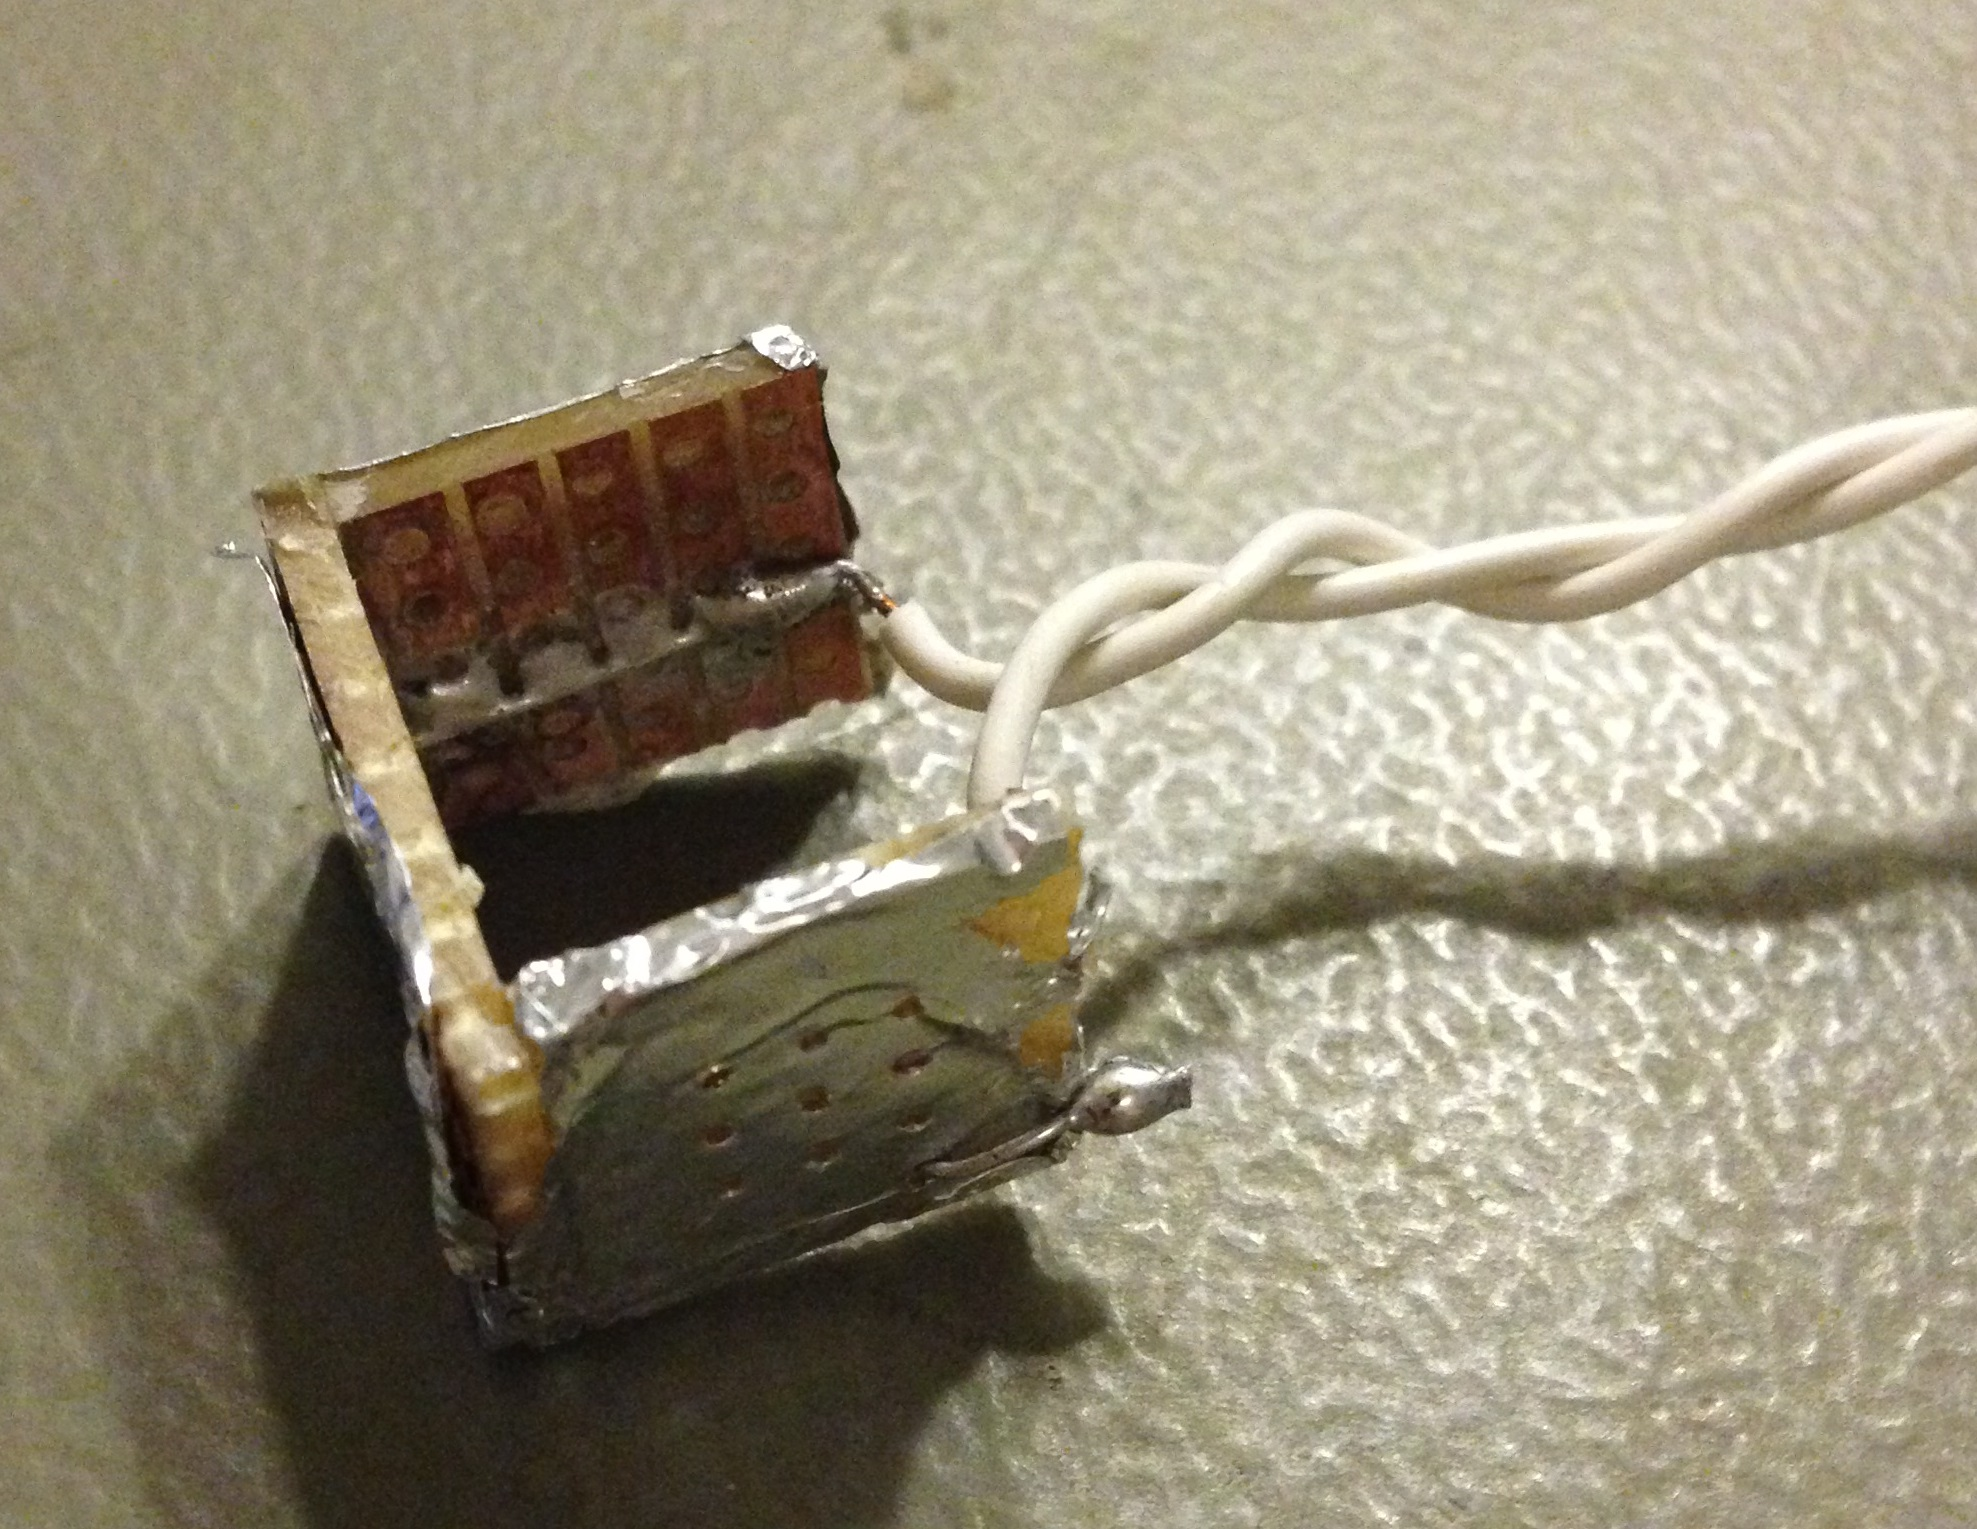
\includegraphics[scale=0.1]{HardwareArkitektur/Sensore/Jordfugt_billeder/Kapacitiv_foler.JPG}
	\caption{Opbygning af den kapacitive f$\text{ø}$ler}
	\label{photo:Kapsitiv_foeler}
\end{figure}

Til den hjemmebyggede pladekondensator blev der også opbygget en oscillator som varierede sin udgangsfrekvens afhængig af kondensatorens kapacitet. Dette kredsløb blev bygget med en LM555. Da pladekondensatoren var en kopi fra det før omtalte pdf dokument kom det ikke som en overraskelse at oscillatoren ændrede sin frekvens med næsten 50\% når pladekondensatoren blev holdt over dampen fra en kop kogende vand. Hvad der dog ikke var taget højde for var kapaciteten i tilledningerne, som ændrede sig hver gang pladekondensatoren blev flyttet. Det viste sig også at når pladekondensatoren blev trykket ned i jord stoppede oscillatoren med at oscillere. Det var hellere ikke muligt at måle kapaciteten med et LCR-meter og ideen blev derfor opgivet. 

\subsection{Resistiv måling}
Næste step var at finde en ny metode til at måle fugtigheden i jorden og denne opstod ved besøg på denne side\footnote{http://gardenbot.org/howTo/soilMoisture/}. \fxnote{tilføjes til literatur liste} På siden bliver det beskrevet hvordan man kan måle fugtigheden i jorden rent resistivt. Desværre bliver der ikke givet nogle værdier på jordens ledeevne i forhold til fugtigheden og var derfor op til en selv at finde den. Ved en størrer søgning blev der fundet frem til oversigten i figur \ref{photo:Ledeevne_grundstoffer} \footnote{Kilde: http://zonge.com/rock-properties-lab/ore-minerals-physical-properties/}\fxnote{tilføjes til litteratur liste}

\begin{figure}[H]
	\centering 
	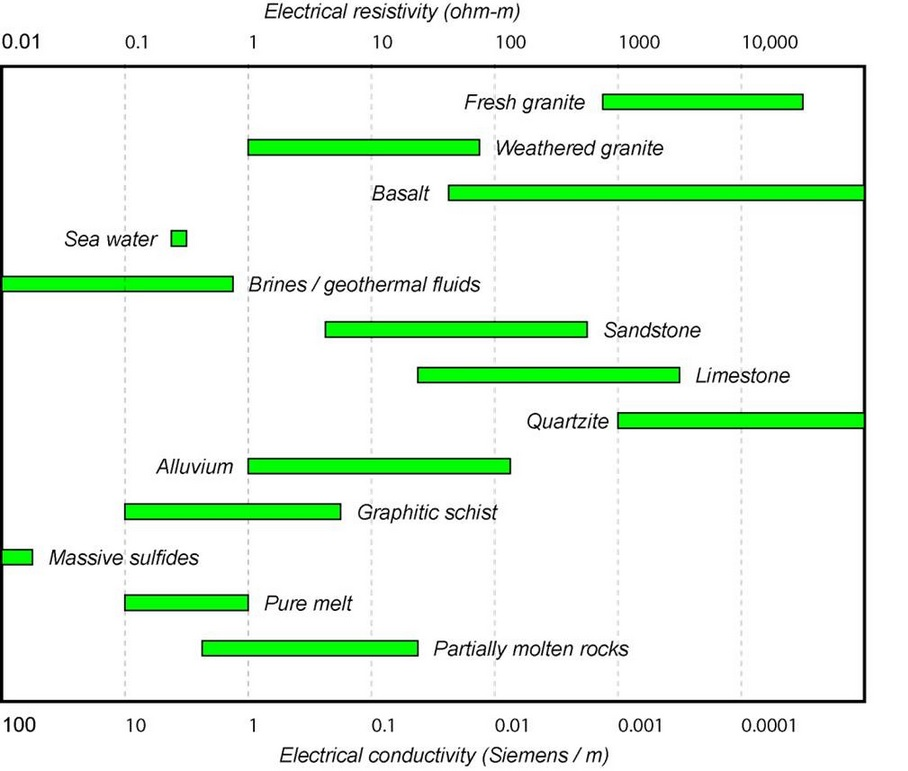
\includegraphics[scale=0.5]{HardwareArkitektur/Sensore/Jordfugt_billeder/soil_conductivity_types.JPG}
	\caption{Oversigt over ledeevnen for nogle forskelige grudstoffer.}
	\label{photo:Ledeevne_grundstoffer}
\end{figure}

Det ses her at Fx. Sandsten varierer fra en ledeevne på 0.5 til 0.003 Siemens/m. Dette er et meget stort spekter og det vil derfor være umuligt at sige noget om ledeevnen i vores jord uden at have målt den. For at kunne gøre dette krævede det at der blev lavet et jordspyd der kunne bruges til at lave målingen med. I figur \ref{photo:Ledeevne_grundstoffer} ses jordspyddet sænket ned i vand fra vandhanen, for at måle vandets ledeevne. Da jordspyddet er isoleret delvist med krympeflex, således at der er et fast areal på begge spyd der er i kontakt med vand vil det være muligt at beregne ledeevnen for vandet.

\begin{figure}[H]
	\centering 
	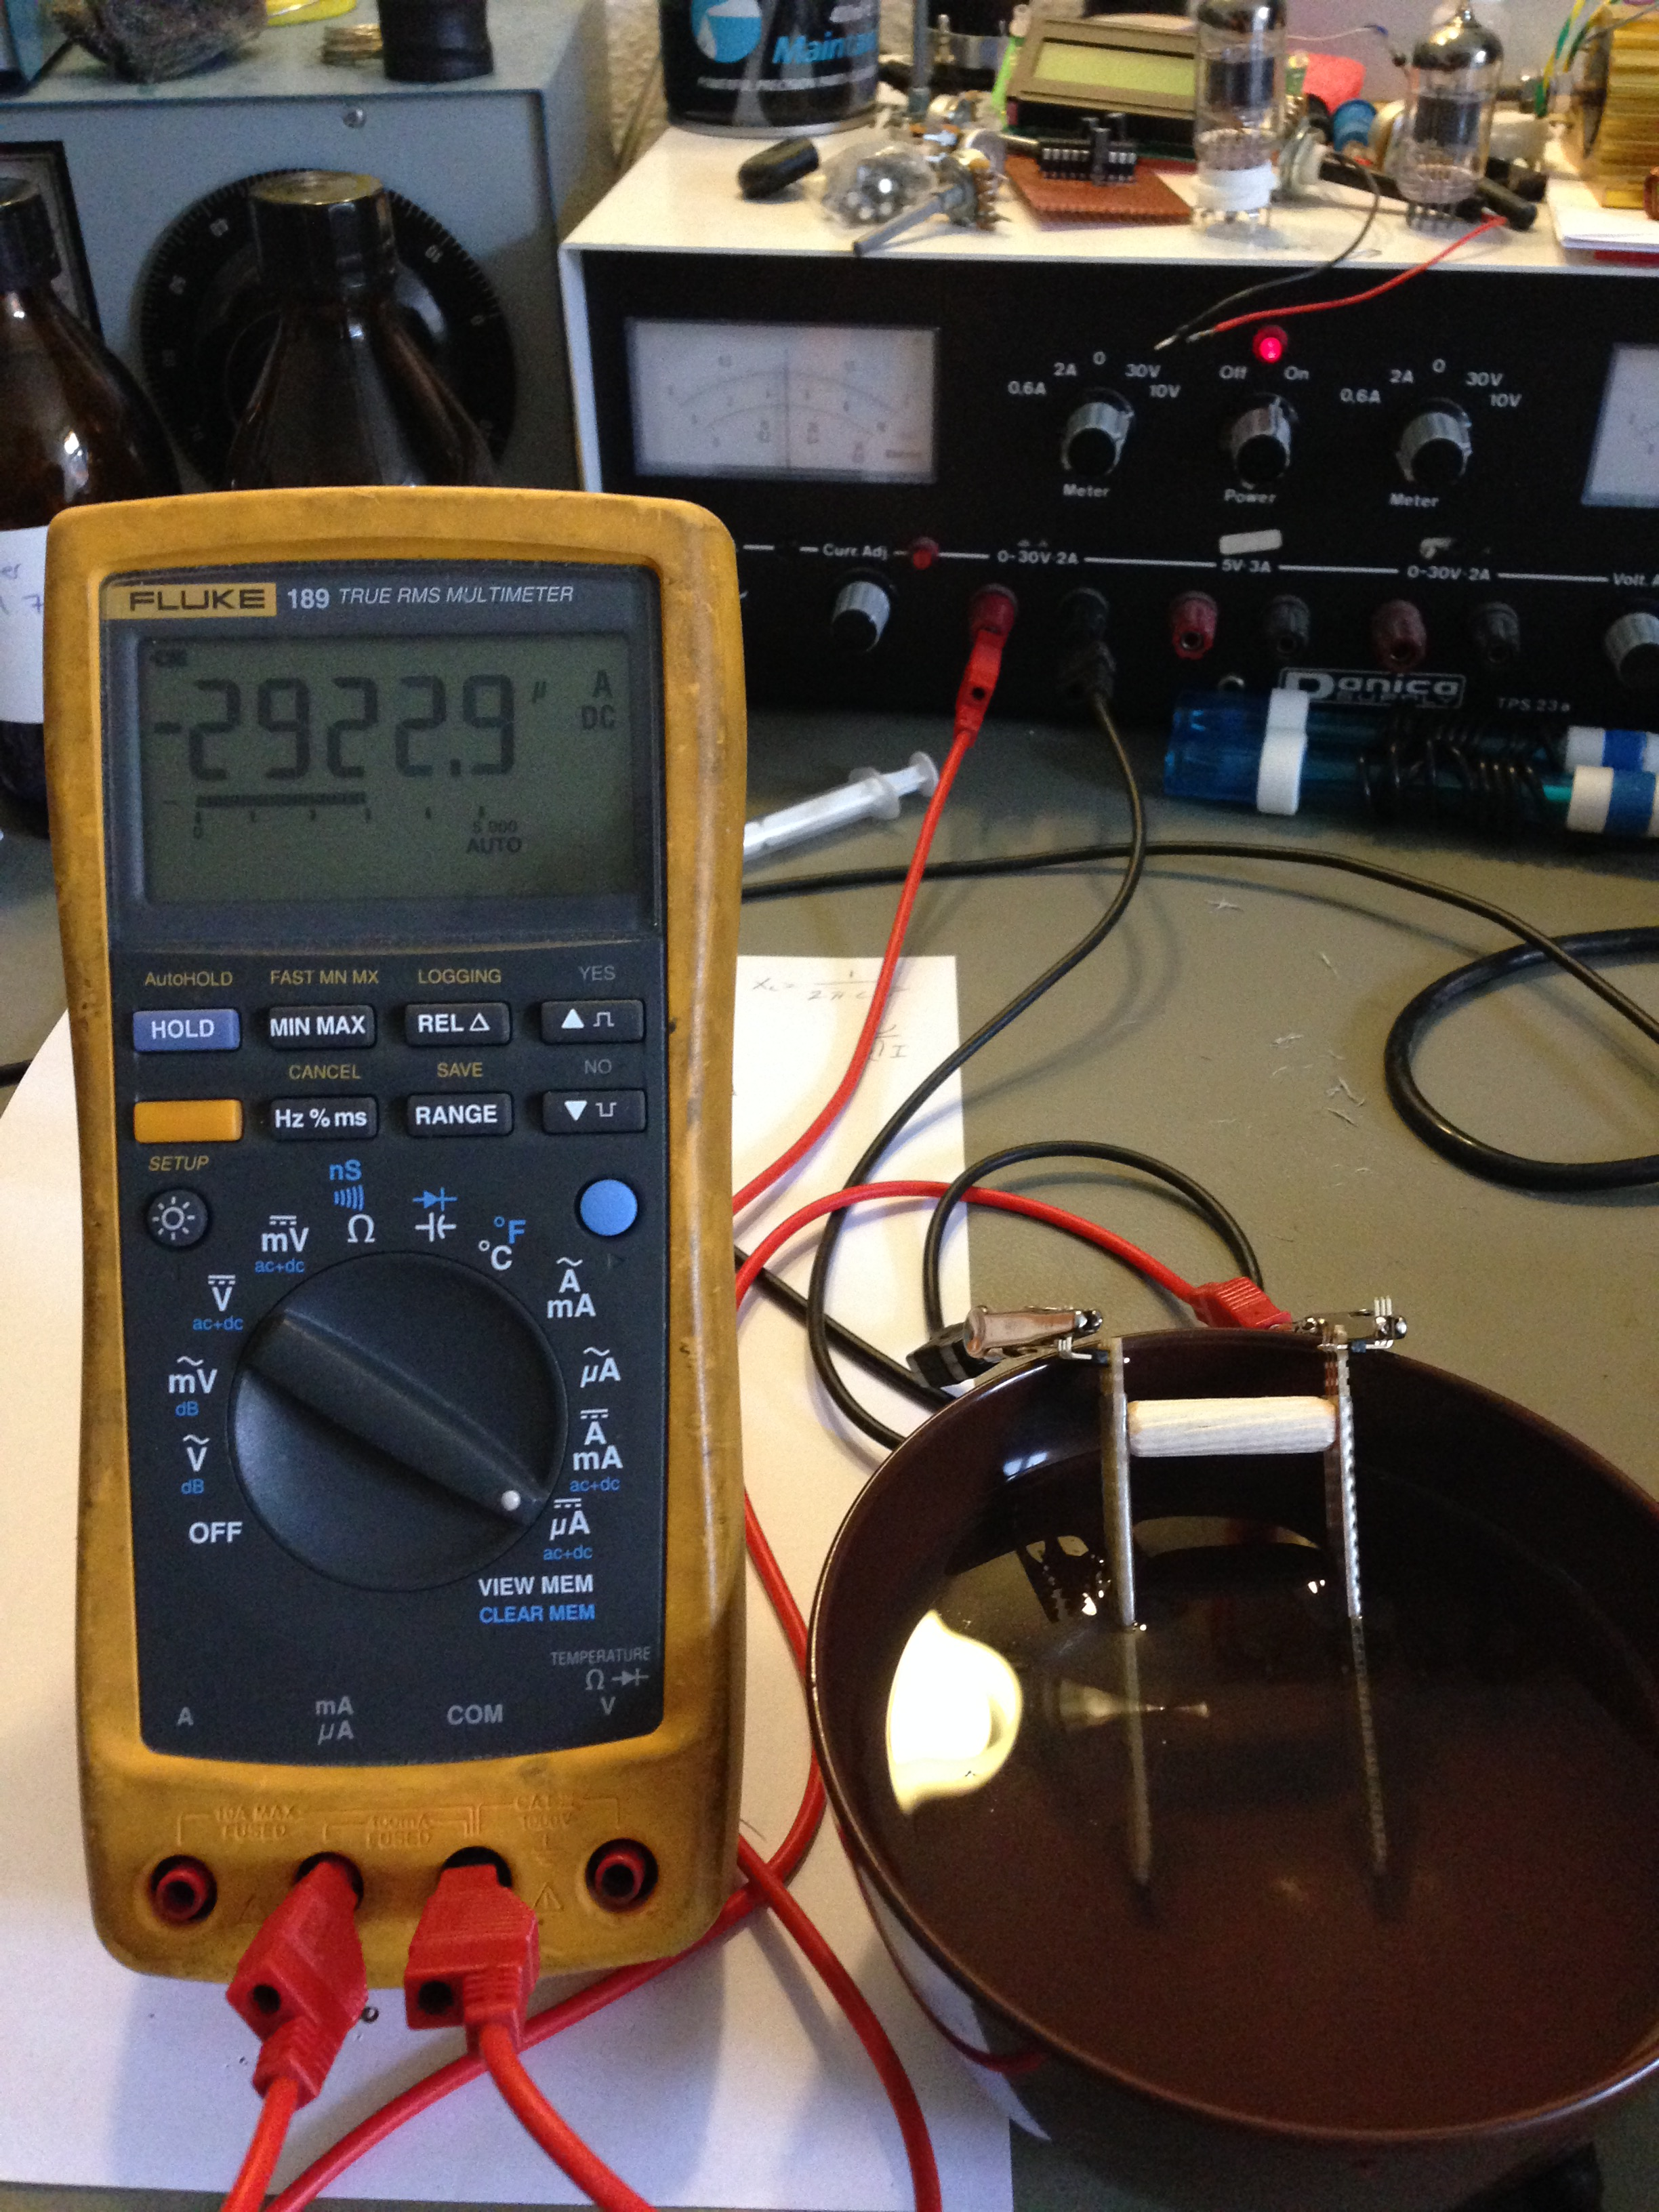
\includegraphics[scale=0.07]{HardwareArkitektur/Sensore/Jordfugt_billeder/Jordspyd_i_vand.JPG}
	\caption{Multimeteret måler strømmen igennem jordspyddet ved en spænding på 5V (2.92mA}
	\label{photo:Jordspyd_vand}
\end{figure}  

\begin{figure}[H]
	\centering 
	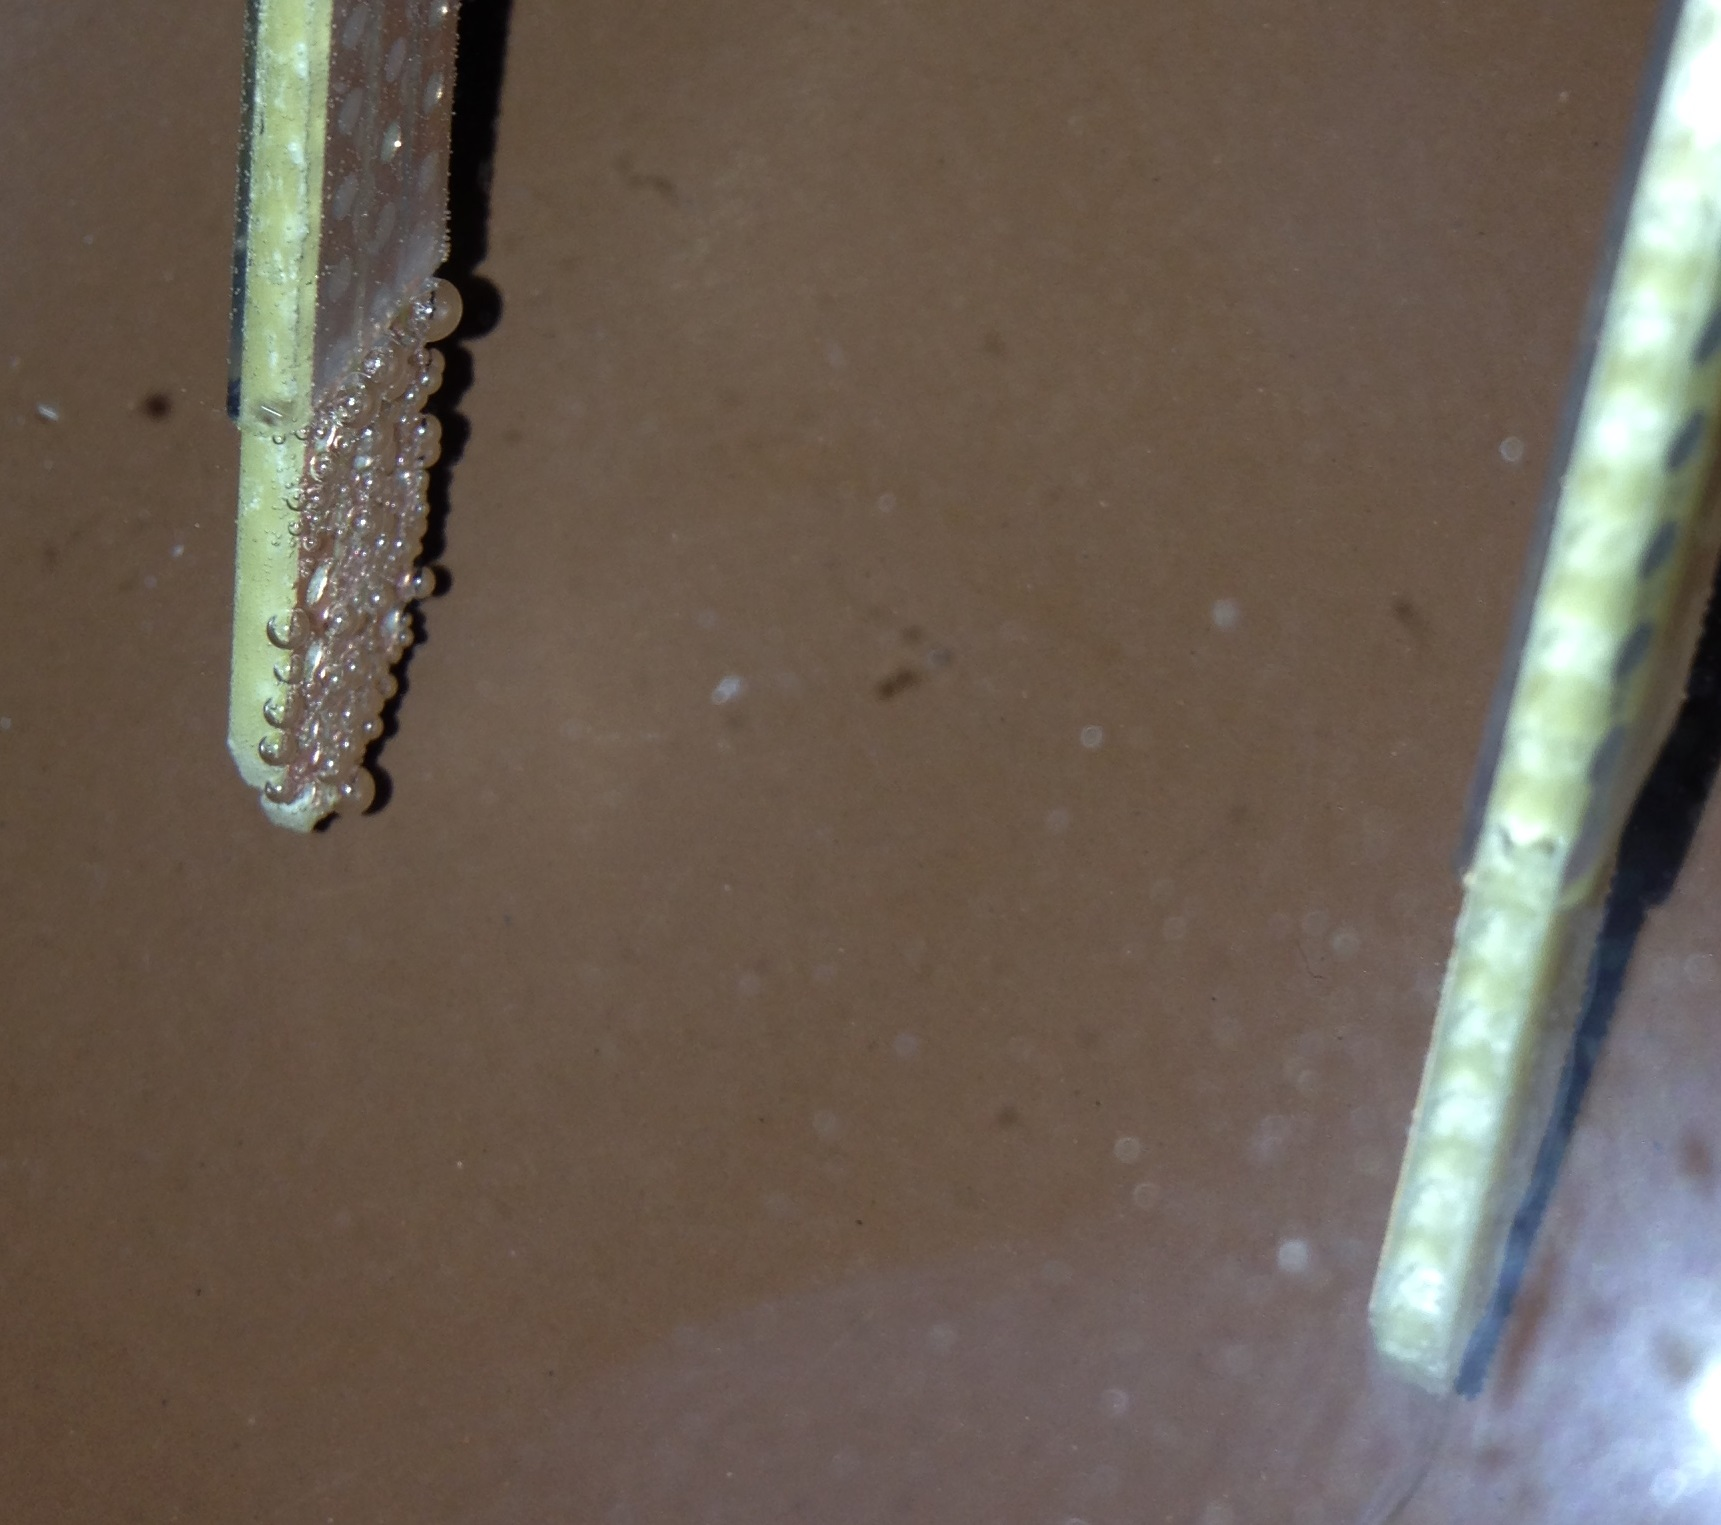
\includegraphics[scale=0.1]{HardwareArkitektur/Sensore/Jordfugt_billeder/Elektrolyse.JPG}
	\caption{Elektrolyse ved 5V}
	\label{photo:Elektrolyse}
\end{figure}  

På figur \ref{photo:Elektrolyse} ses at der desværre også forekommer elektrolyse ved denne målemetode. Der ses at katoden tiltrækker hydrogen atomer som sætter sig som luftbobler på kobberet. Ved en spænding på 30V var elektrolysen så kraftigt at kobberlaget på anoden ville være væk efter få minutter. Derfor konstanters det også at ved implementering af denne type måling må der kun gå strøm i jordspyddet i det øjeblik målingen bliver foretaget, for at undgå unødvendig slid. 
\\*
\\*
Den mest interessante opdagelse blev gjort ved målingen af jorden. Her var teorien at ledeevnen ville stige lineært med fugtigheden. Det viste sig at være forkert og det lignede i stedet et fjerdegrads stigene polynomium, da måleresultaterne blev tegnet ind i Graph. Forinden havde det været et stort problem at finde ud af hvilken skala der skulle bruges til at måle fugtigheden, da der findes mange definitioner af den. Der blev fundet frem til at fugtigheden i tørvægt var den mest brugbare for geoteknikere og der var derfor den skala der blev valgt. Skalaen siger at hvis der er 100 gram ovntørret jord og 40 gram vand indeholder jorden 40\% fugtighed. I formlen står m for masse.
$$ \mu = \frac{m_{wet}-m_{dry} }{m_{dry}}$$ 
\\*
\\*
I figur \ref{photo:Opvejning} og \ref{photo:Maetningspunkt} ses hvordan målingerne af jordfugtigheden blev foretaget. 

\begin{figure}[H]
	\centering 
	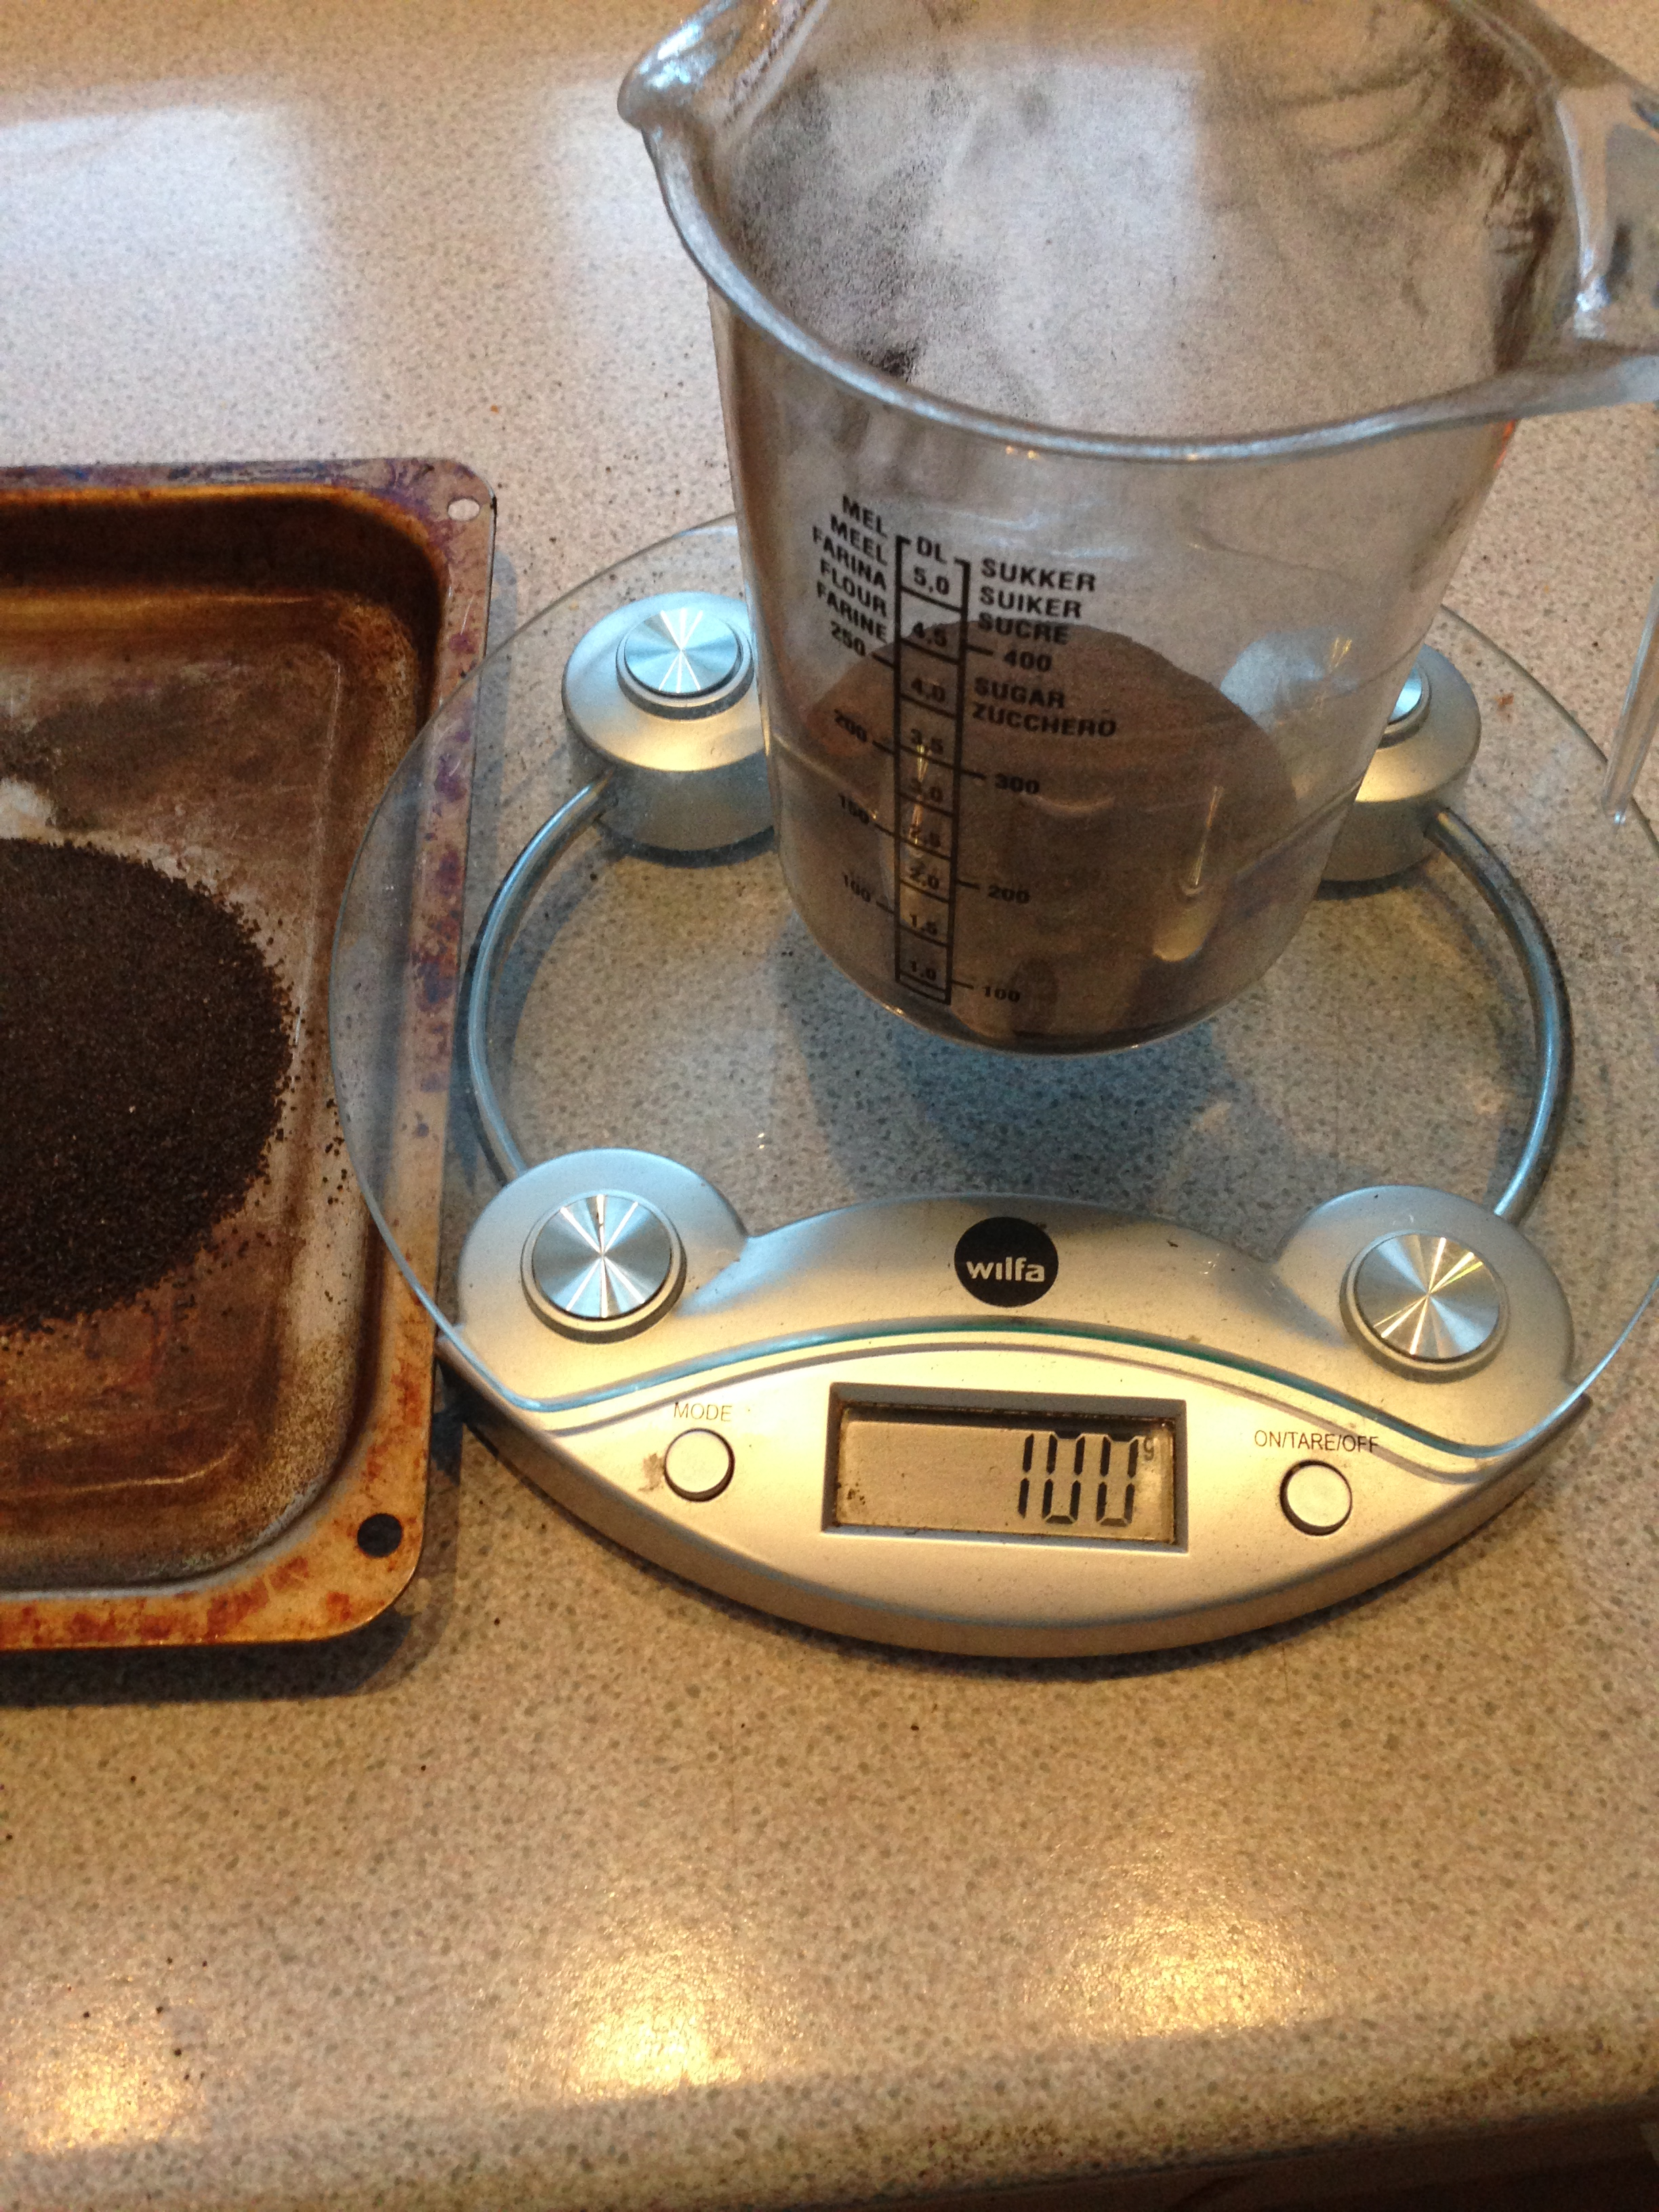
\includegraphics[scale=0.08]{HardwareArkitektur/Sensore/Jordfugt_billeder/Opvejning.JPG}
	\caption{Vejning af 100 gram af ovntørret jord. Vægten er nulstillet med tomt målebægre}
	\label{photo:Opvejning}
\end{figure}  
 
\begin{figure}[H]
	\centering 
	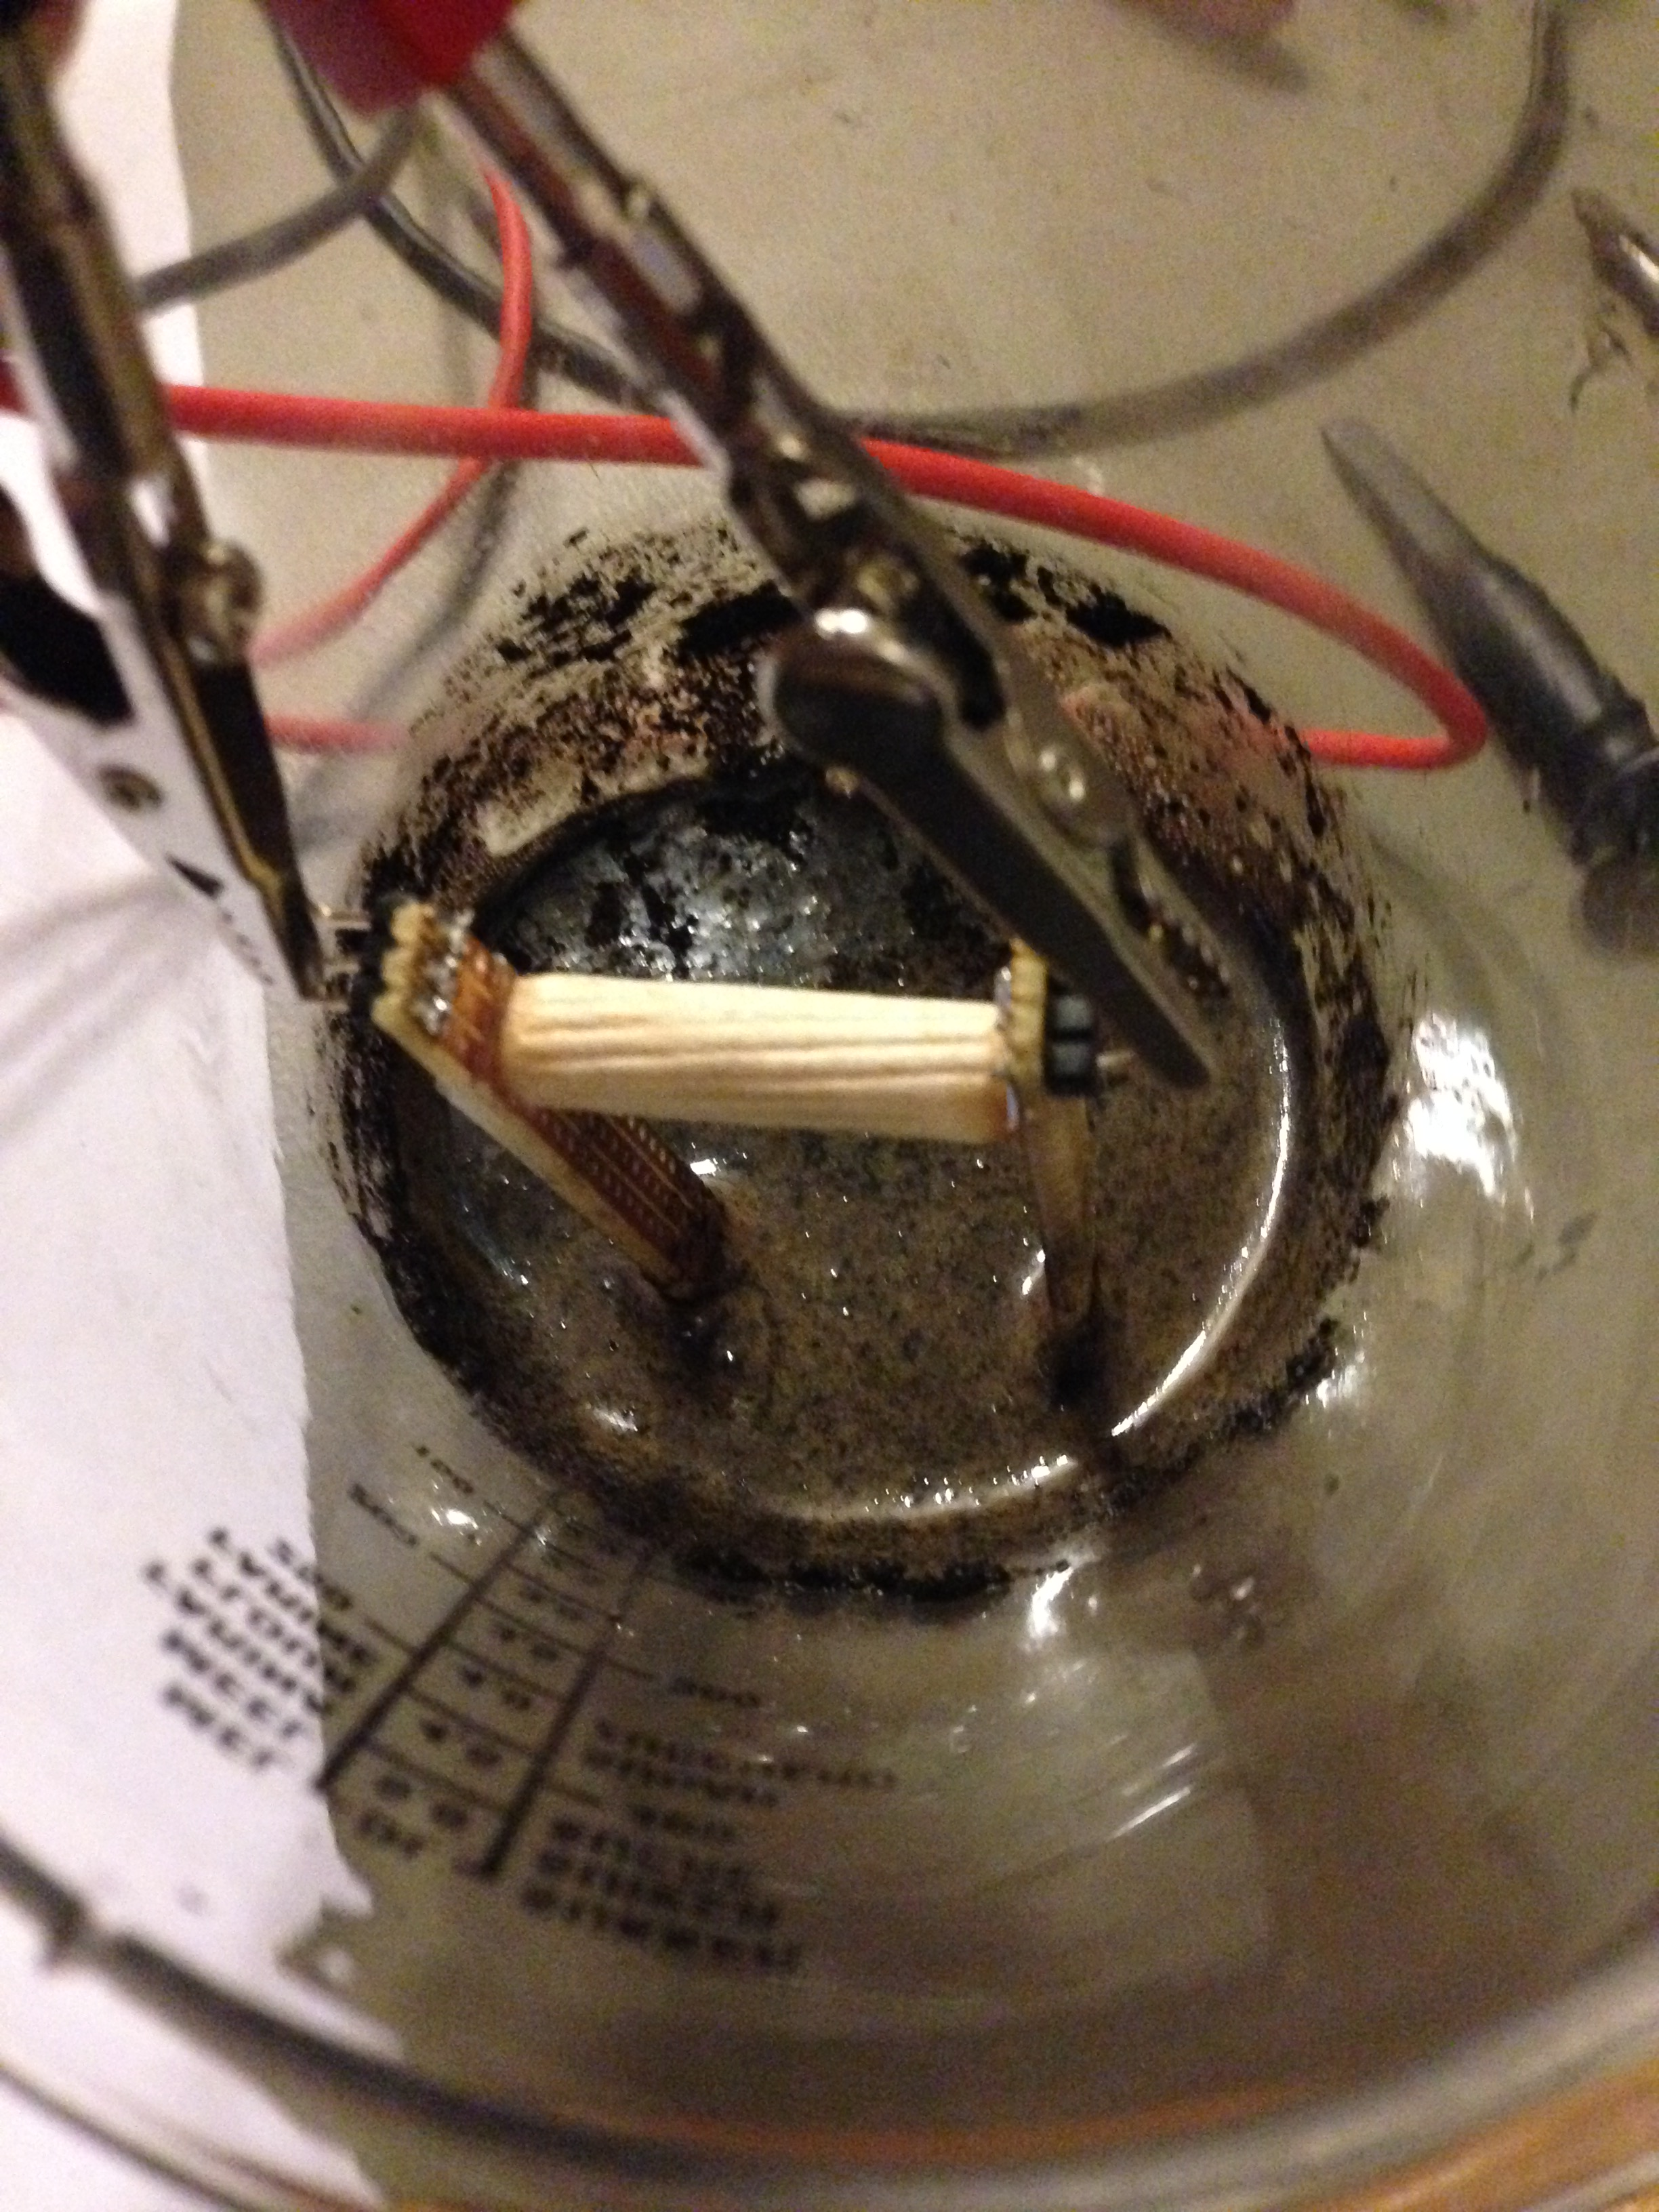
\includegraphics[scale=0.08]{HardwareArkitektur/Sensore/Jordfugt_billeder/Maetningspunktet.JPG}
	\caption{Her ses blandingsforholdet hvor strømmen i jordspyddet igen er faldende}
	\label{photo:Maetningspunkt}
\end{figure}  

I figur \ref{photo:Maetningspunkt} blev der lavet 7 målinger ved forskellig fugtighed. Ved en fugtighed på 25.6\% begyndte strømmen i jordspyddet at falde igen. Dette bliver et problem i det samlede system da systemet ikke kan vide om den måler i en overvandet plante. figur \ref{photo:Graph_jordfugtighed}. Viser regression af målepunkterne. 

\begin{figure}[H]
	\centering 
	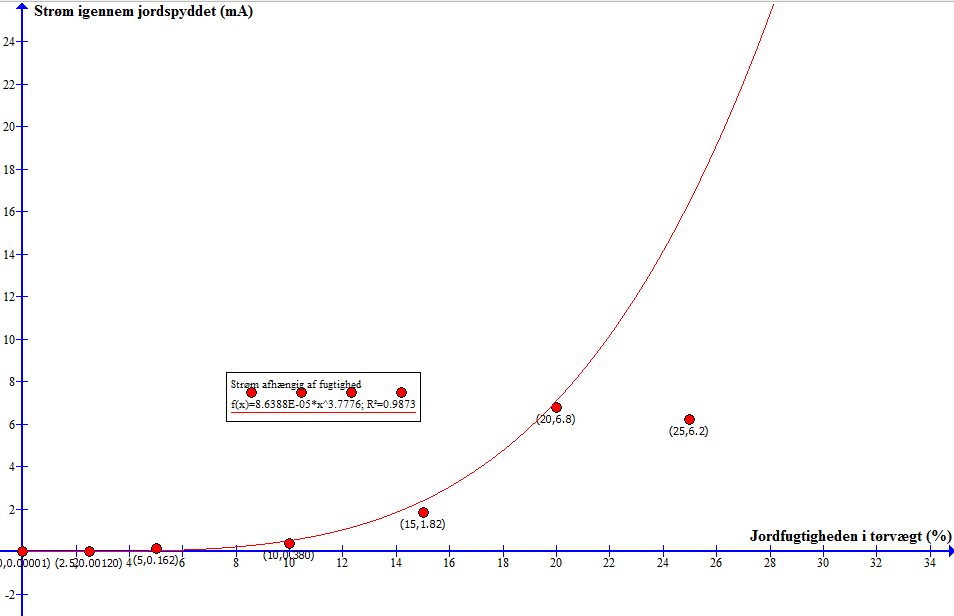
\includegraphics[scale=0.6]{HardwareArkitektur/Sensore/Jordfugt_billeder/Graph_jordfugtighed.PNG}
	\caption{Målinger indtegnet i Graph. Den yderste måling til højre (25,6.2) er det før omtalte "knæk punkt" hvor vi ikke længere ved om vi måler rigtigt. punktet er ikke medtaget i regressionen.}
	\label{photo:Graph_jordfugtighed}
\end{figure}  

I figur \ref{photo:Graph_jordfugtighed} aflæsete vi regressionen af graften til at være:
$$f(x) = 8.64*10^{-5}x^{3.77} $$
Funktionen er udtrykket for strømmen i jordspyddet ved en given fugtighed. Dette kan med fordel omskrives til modstand ved brug af ohms lov. Den påtrykte spænding fra spændingsgeneratoren var 5V
$$f(x) = \frac{5V}{{8.6388*10^{-5}*x^{3.78}*10^{-3}A}}$$
Denne funktion kan bruges i en mikroprocessor med en analog til digital konverter, således strømmen kan omregnes til jordfugtigheden i procent.På figur \ref{photo:jordspyd_modstand} ses grafen over funktionen. 

\begin{figure}[H]
	\centering 
	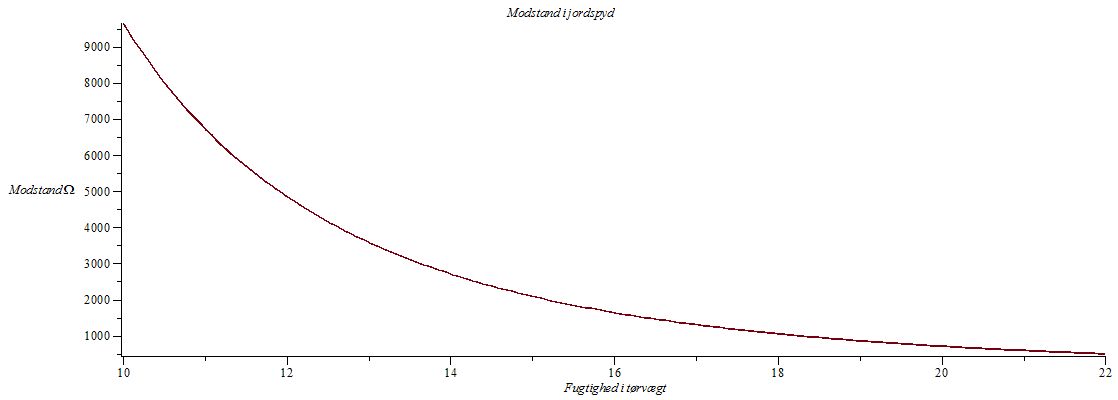
\includegraphics[scale=0.4]{HardwareArkitektur/Sensore/Jordfugt_billeder/jordspyd_modstand.PNG}
	\caption{Plot over modstanden i jordspyddet ved en given fugtighed.Grafen er et udsnit fra 10\% til 22\% for at gøre den mere overskuelig}
	\label{photo:jordspyd_modstand}
\end{figure}  

\subsection{Test og opbygning}
Næste punkt var at finde en metode til at måle modstanden i spyddet. Dette kunne gøres ved at koble jordspyddet som en spændingsdeler med en MOSFET transistor til at lede strømmen når der måles. På figur \ref{photo:jordspyd_diagram} ses diagrammet over forklaringen. 
 
\begin{figure}[H]
	\centering 
	\includegraphics[scale=0.8]{HardwareArkitektur/Sensore/Jordfugt_billeder/jordspyd.JPG}
	\caption{Diagram over jordspyddet}
	\label{photo:jordspyd_diagram}
\end{figure} 

Der opstilles følgende funktion for kredsløbet:
$$Rspyd=-{\frac {{Vout}\,{R1}}{{Vout}-{Vcc}}}$$
Ved at isolere x ud fra funktionen på figur \ref{photo:jordspyd_modstand} kan vi få et udtryk for fugtigheden hvis vi kender modstanden. 
$$fugt=\frac{113.47}{Rspyd^{0.26472}}$$
Disse to formler blev brugt i PSoC creator til at programmere en CY8C4245AXI-483 med en differentiel koblet analog til digital konverter. På figur \ref{photo:ADC} ses topdesignet i PSoC creator.    

\begin{figure}[H]
	\centering 
	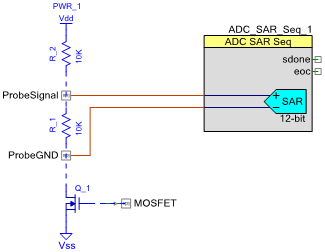
\includegraphics[scale=0.8]{HardwareArkitektur/Sensore/Jordfugt_billeder/SAR_converter.png}
	\caption{Topdesign i PSoC creator}
	\label{photo:ADC}
\end{figure} 

I PSoC creator laves der en funktion der udlæser værdien fra ADC'en og omregner den til fugtighed. På et fumleboard opbygges der et kredsløb med et 4.7k potientometer og en 100ohms modstand koblet serielt. I fugur \ref{photo:debug100} ses debugging af første opbygning af funktionen.

\begin{figure}[H]
	\centering 
	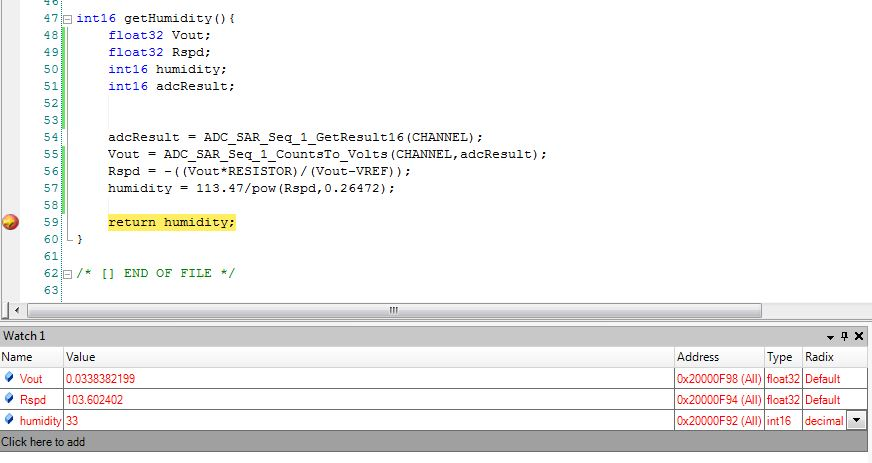
\includegraphics[scale=0.8]{HardwareArkitektur/Sensore/Jordfugt_billeder/debug100ohm.jpg}
	\caption{Debugging i PSoC creator ved Rspyd=100$\Omega$}
	\label{photo:debug100}
\end{figure} 

Aflæser vi 100$\Omega$ på figur \ref{photo:jordspyd_modstand} kan vi se at en fugtighed på 33 stemmer fint overens med det forventede og funktion antages efter flere ligende resultater at virke. Efterfølgende er funktionen lavet om således den også kommunikerer med sensor ø'en. Den færdige kode fildes i bilagende. 

Efterfølgende blev der tegnet et diagram i DesignSpark og der blev i samme program tegnet et printlayout. Dette ses på figur \ref{photo:Print_2} og \ref{photo:Print_2}.

\begin{figure}[H]
	\centering 
	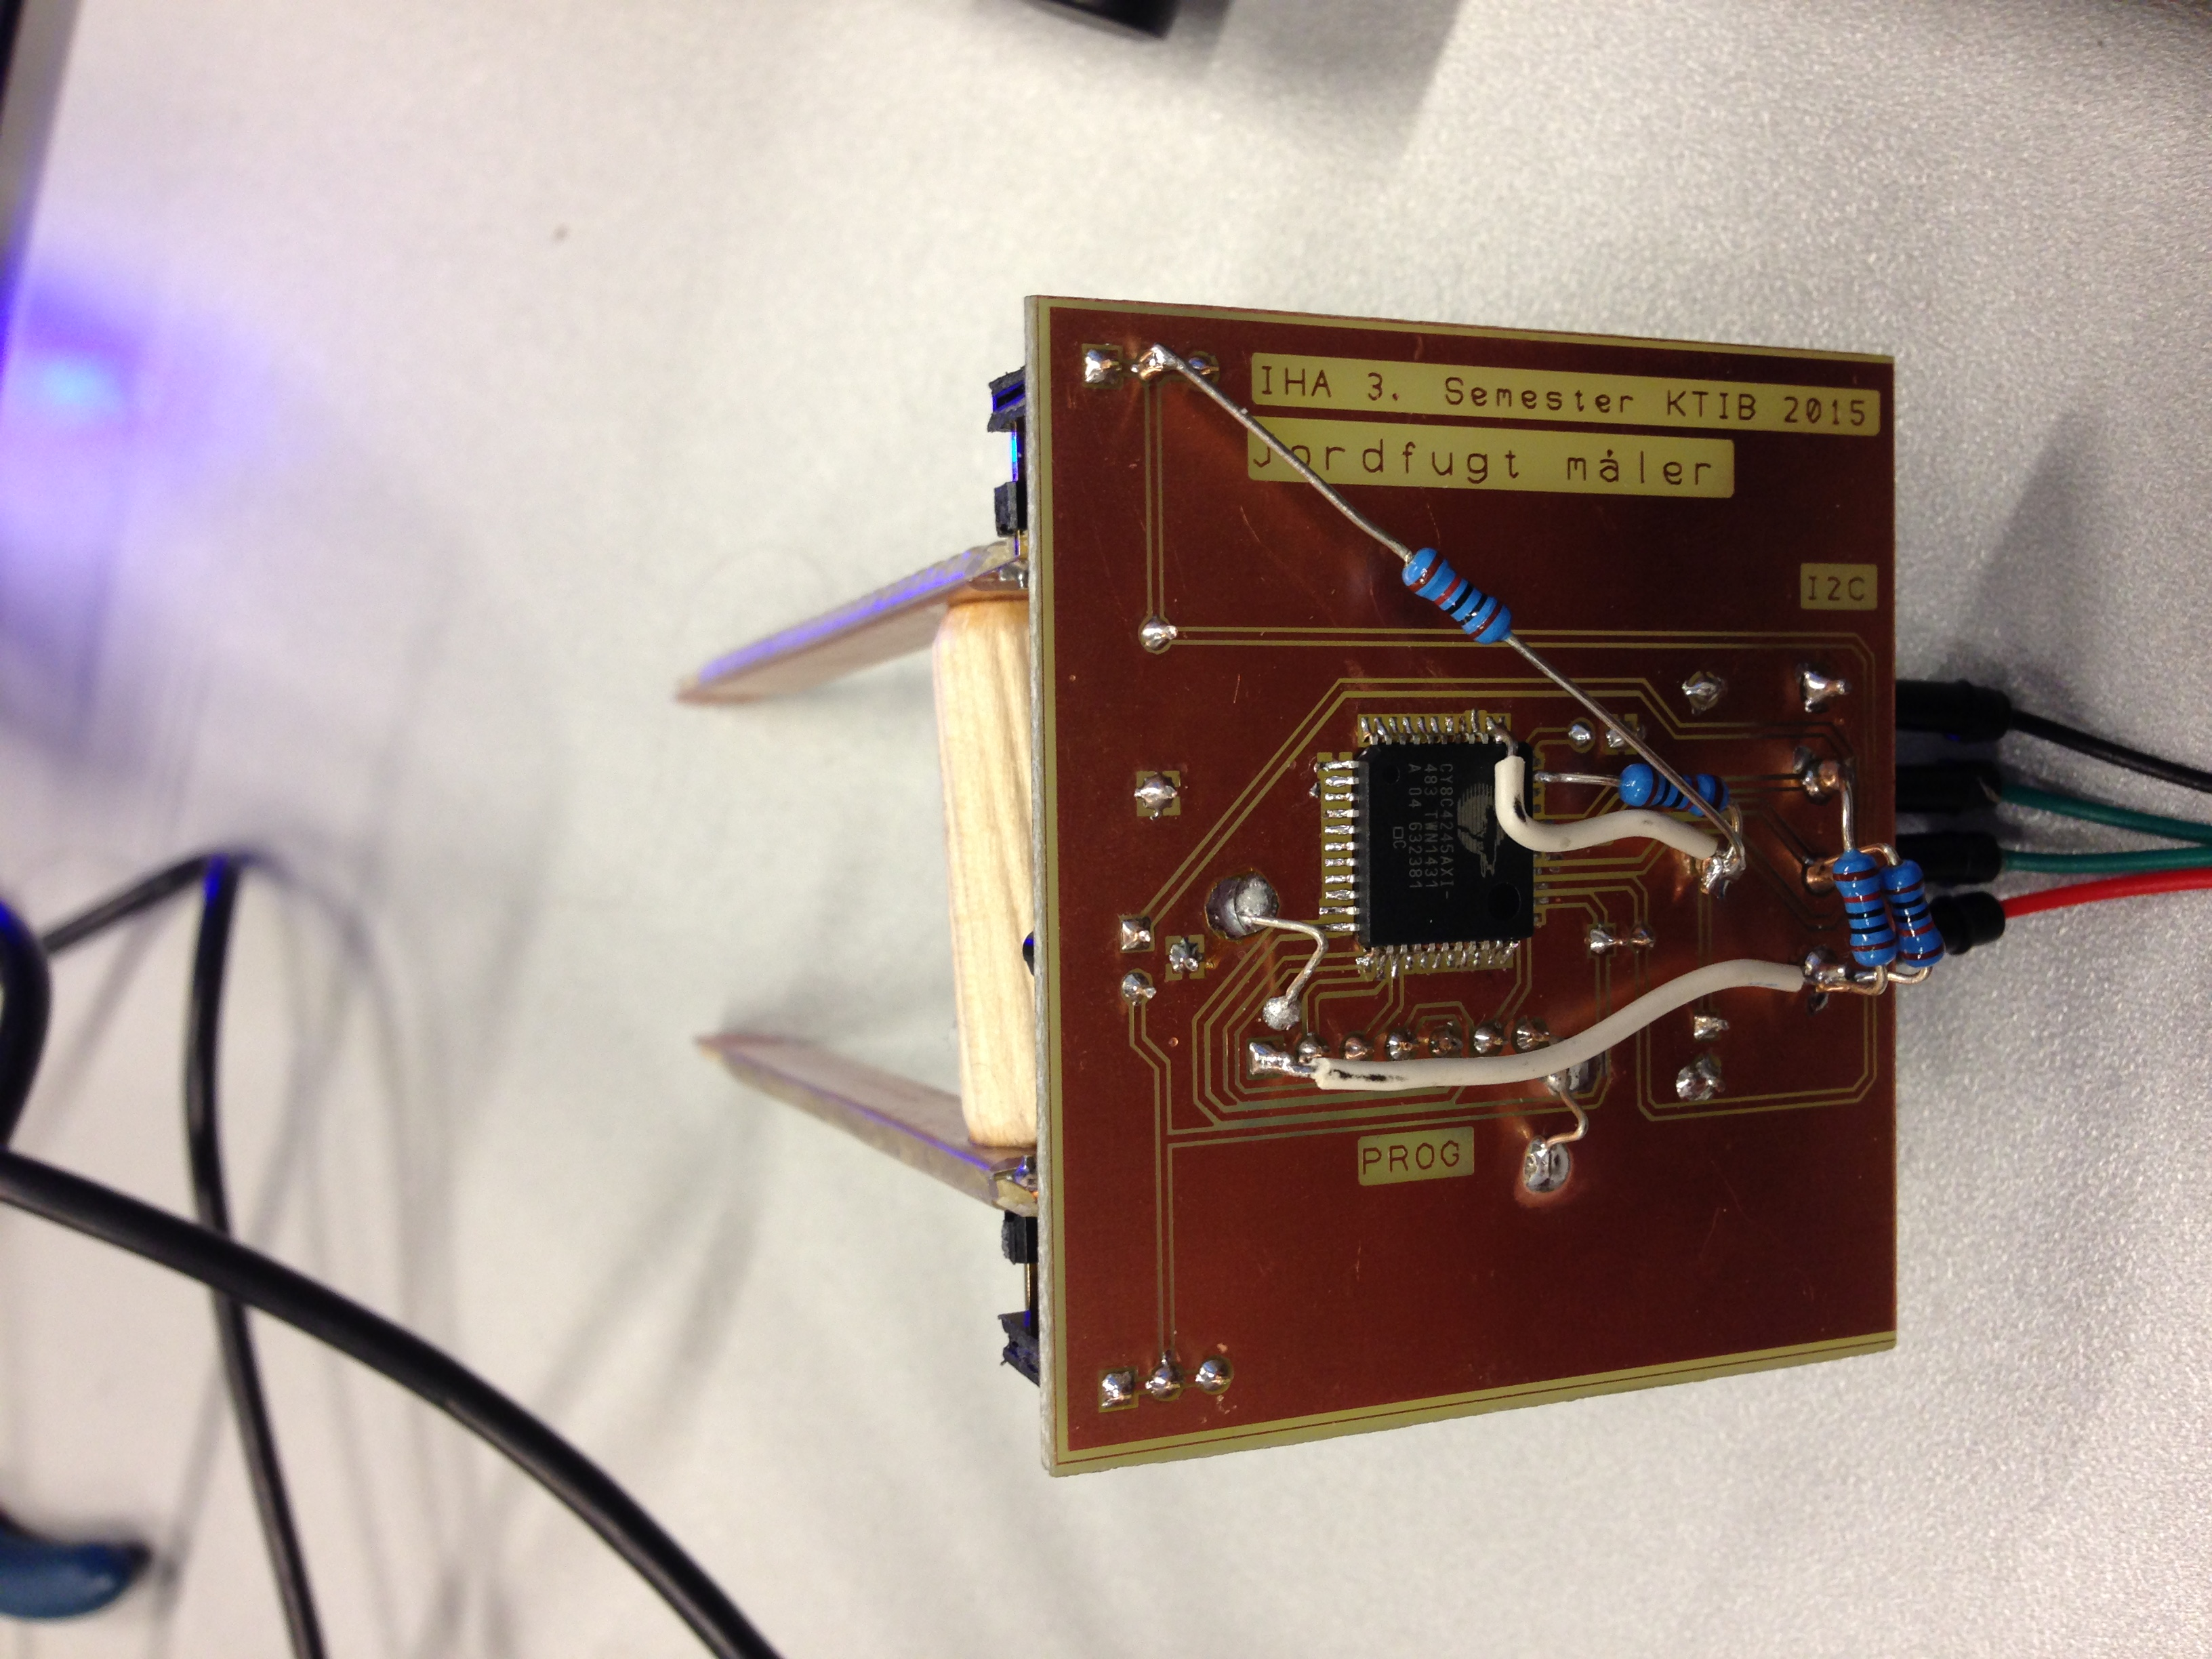
\includegraphics[scale=0.1]{HardwareArkitektur/Sensore/Jordfugt_billeder/Print_2.jpg}
	\caption{Printplade set fra bunden}
	\label{photo:Print_2}
\end{figure} 

\begin{figure}[H]
	\centering 
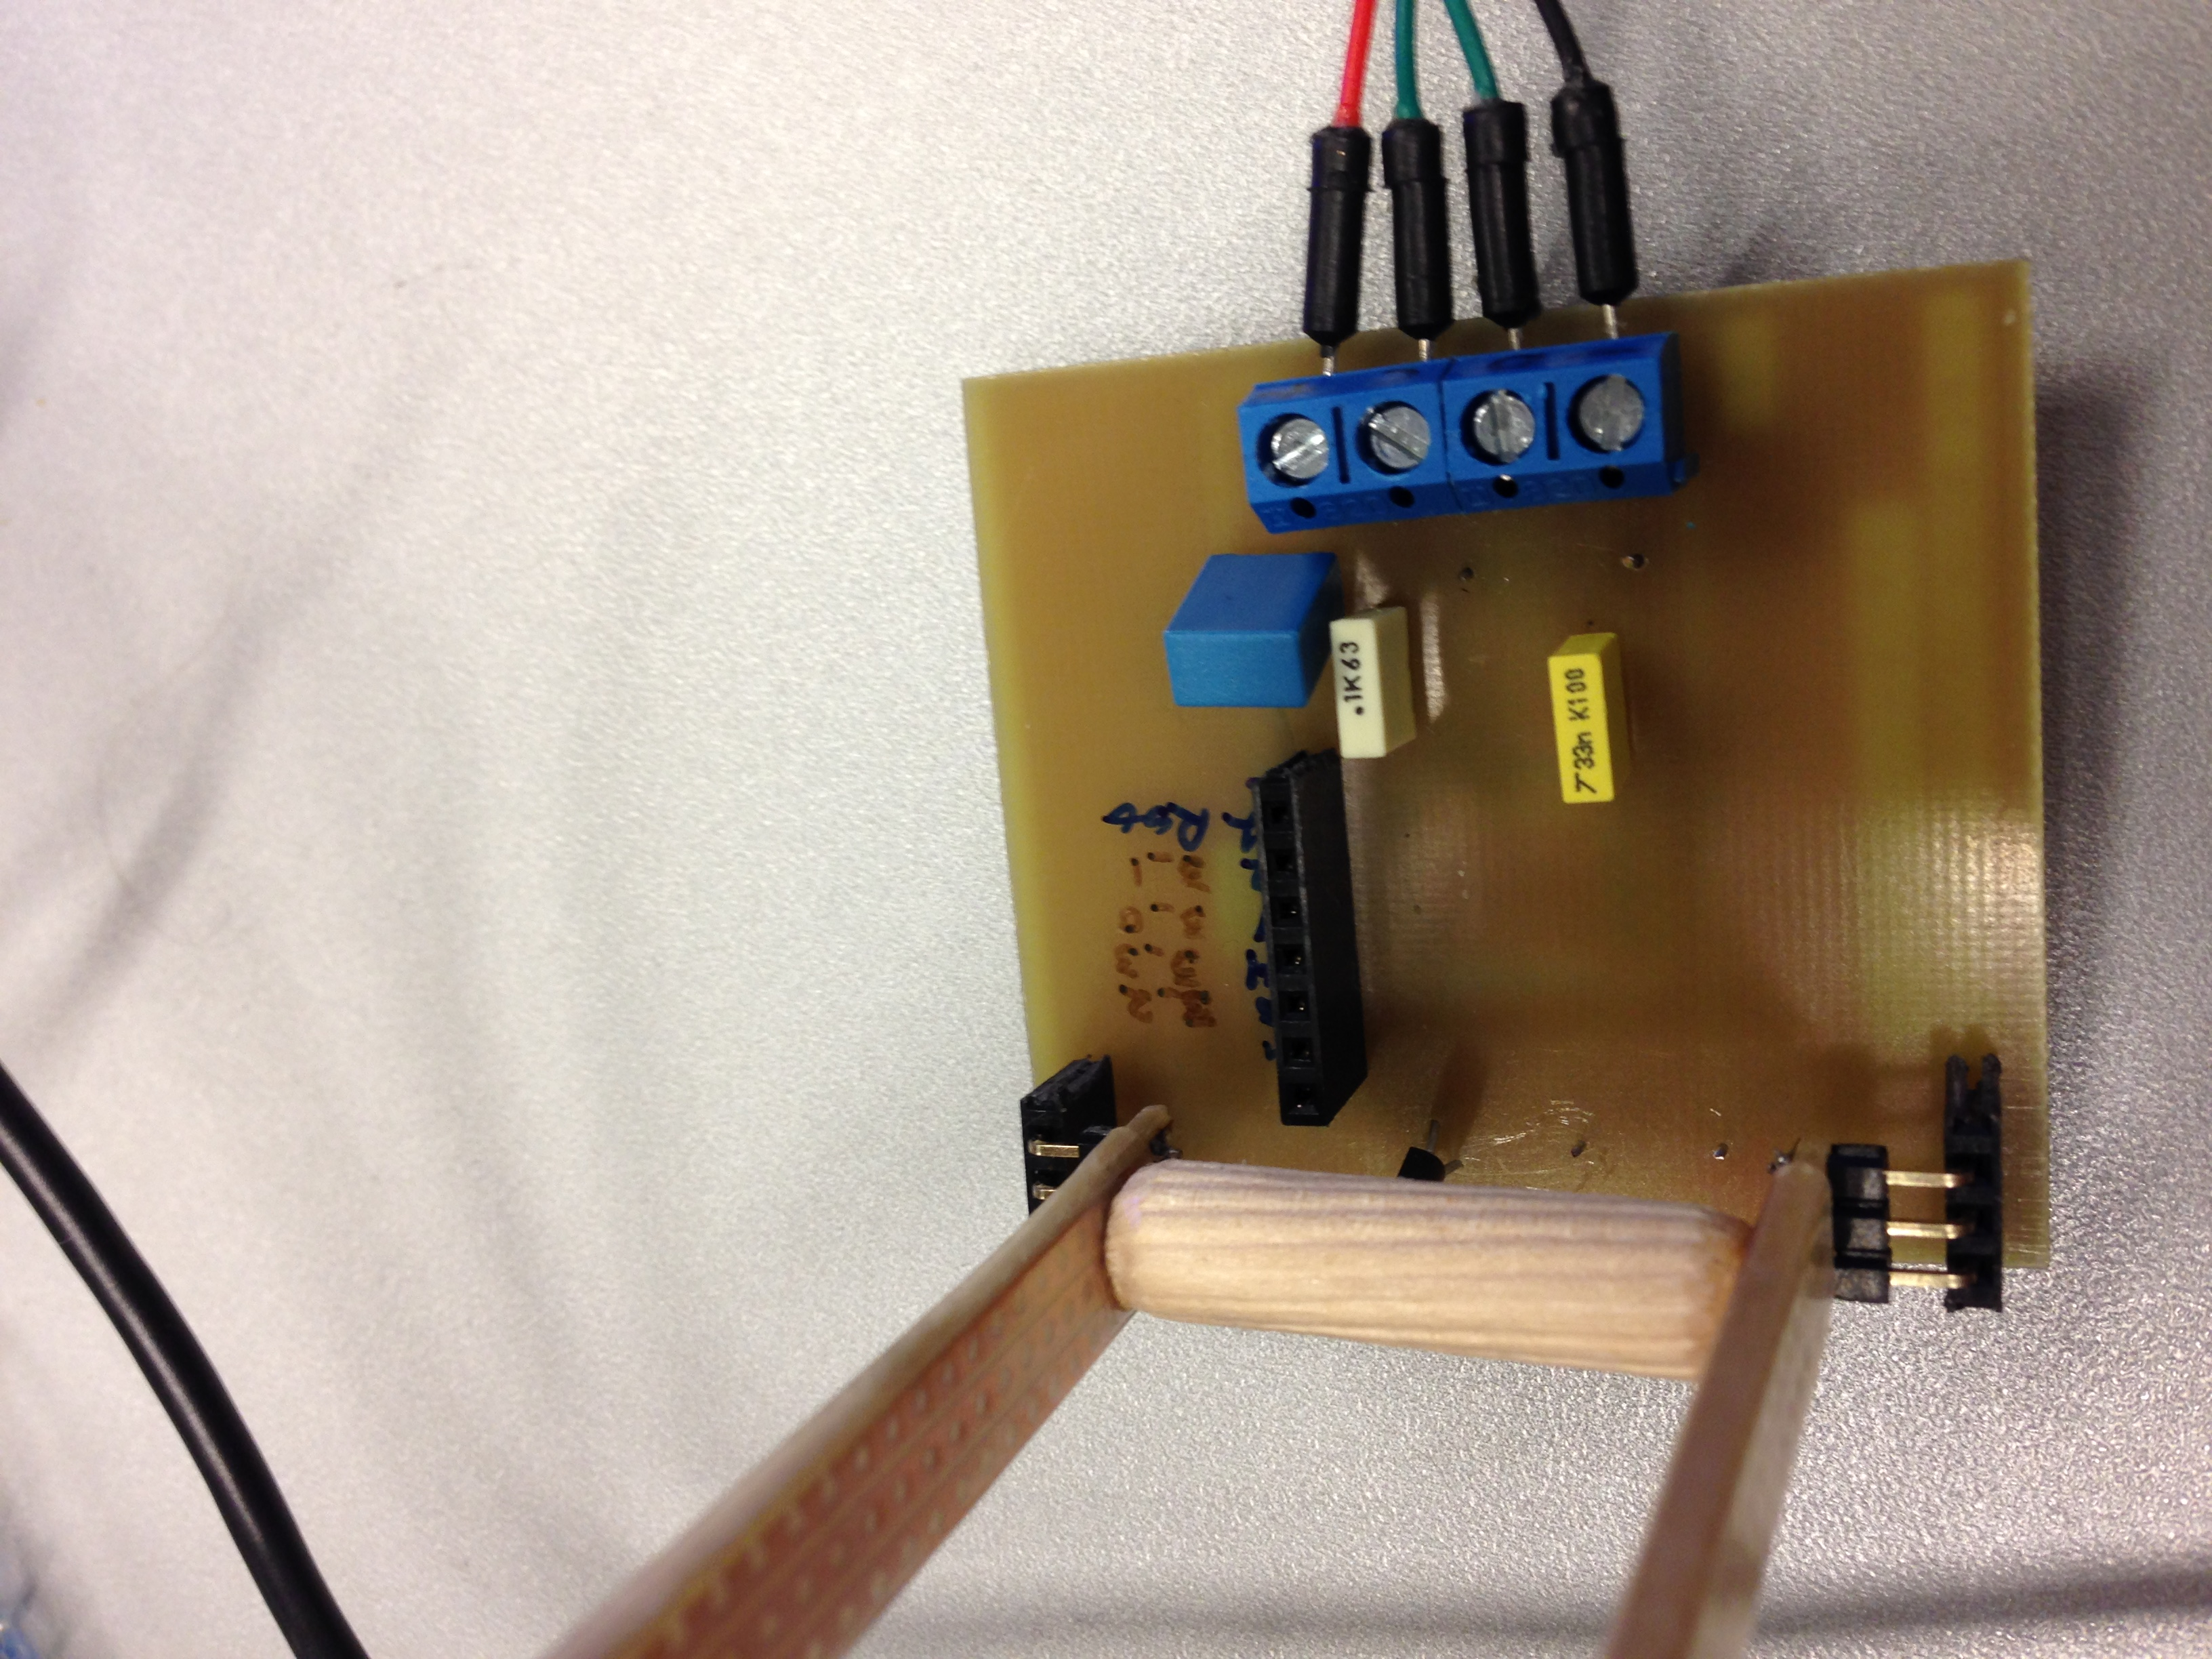
\includegraphics[scale=0.1]{HardwareArkitektur/Sensore/Jordfugt_billeder/Print_1.jpg}
	\caption{Printplade set fra overfladen}
	\label{photo:Print_1}
\end{figure} 

Det ses på printet at der er blevet lavet nogle modifikationer. Dette skyldes at der var glemt nogle pull op modstande, samt at DesignSpark havde valgt at ligge stel sammen med forsyningen. 
Diagrammet blev derfor tegnet om til følgende i figur \ref{photo:Diagram_jordfugt} 

\begin{figure}[H]
	\centering 
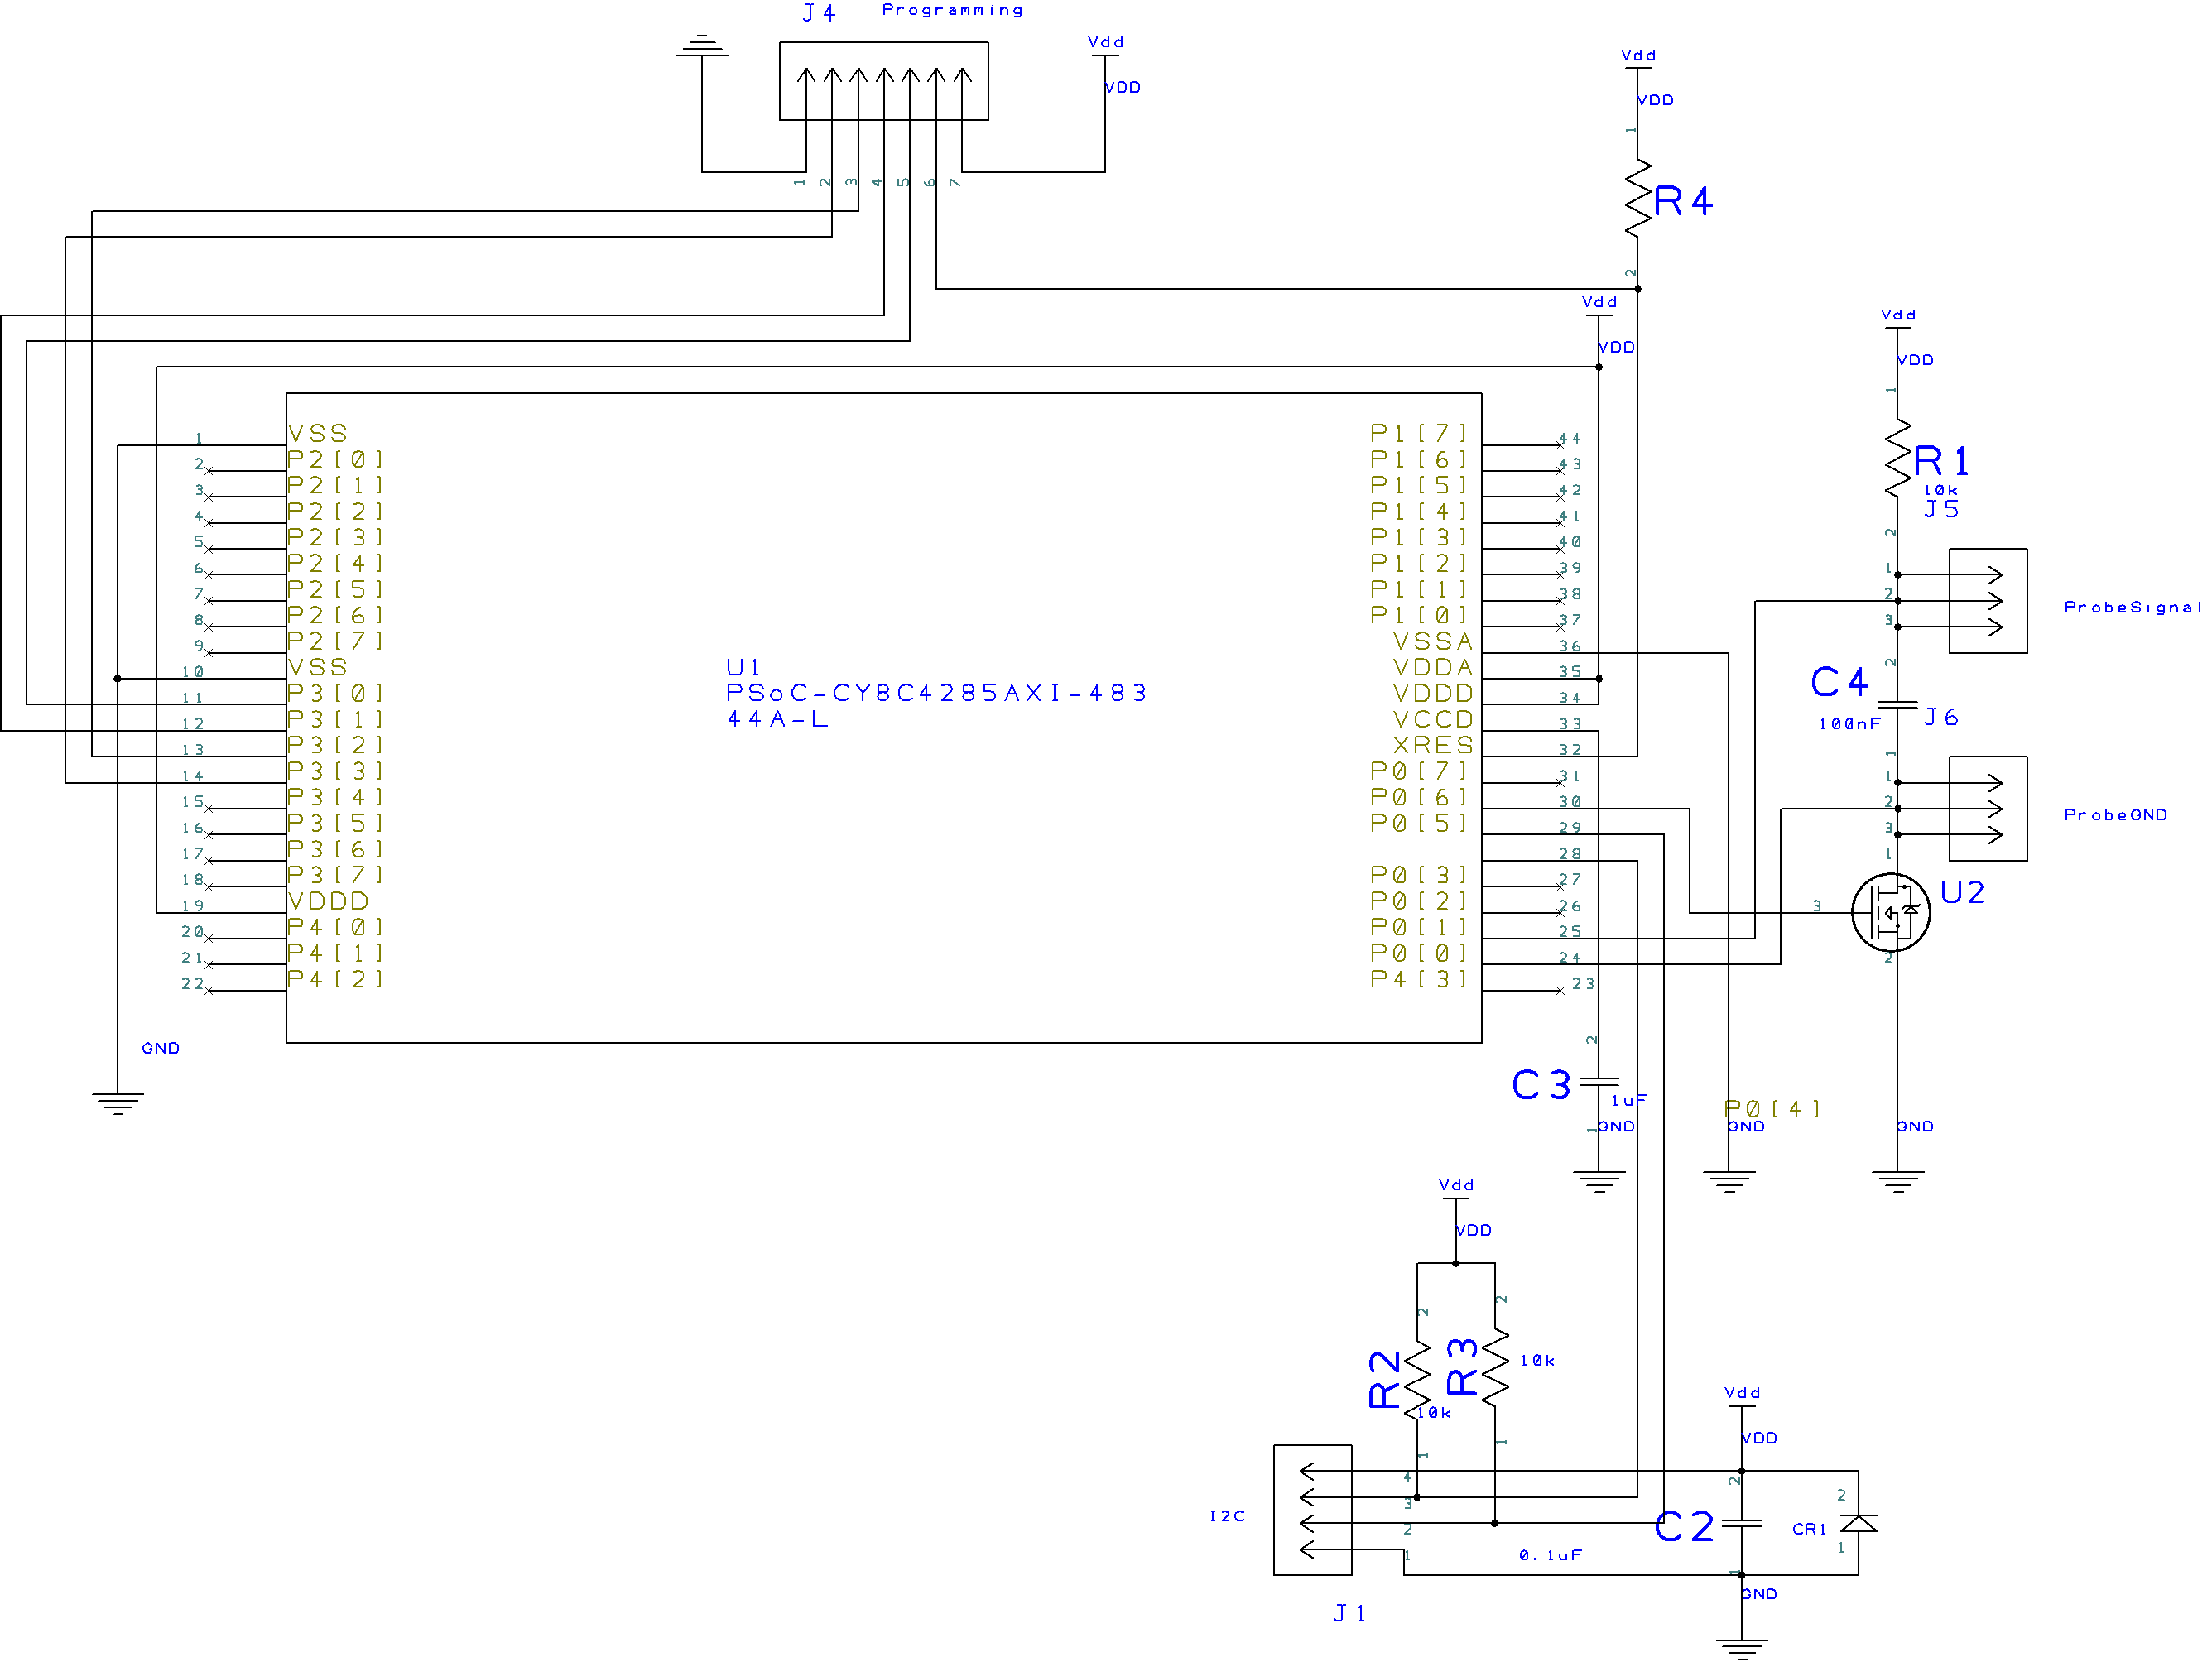
\includegraphics[scale=0.2]{HardwareArkitektur/Sensore/Jordfugt_billeder/Diagram_jordfugt.png}
	\caption{Diagram over jordfugtmåleren}
	\label{photo:Diagram_jordfugt}
\end{figure} 

Det ses på diagrammet i figur \ref{photo:Diagram_jordfugt} at der er trukket stik ud til at programmere PSoC'en. Ved at forbinde disse til vores Pioneer kit kan vi programmere PSoC'en igennem en PSoC 5 og på den måde undgå at skulle købe en programmeringsenhed. Det viste sig dog at der var flere problemer da det nye print blev lavet. Vi kunne sagens kommunikere med PSoC'en igennem programmerings stikket. Men det var umuligt at få nogen funktionalitet ud af den. Der blev brugt dage på at finde ud af hvad der kunne være galt, uden resultat. Det blev derfor besluttet at lave et shield til pioneer kittet. 

\begin{figure}[H]
	\centering 
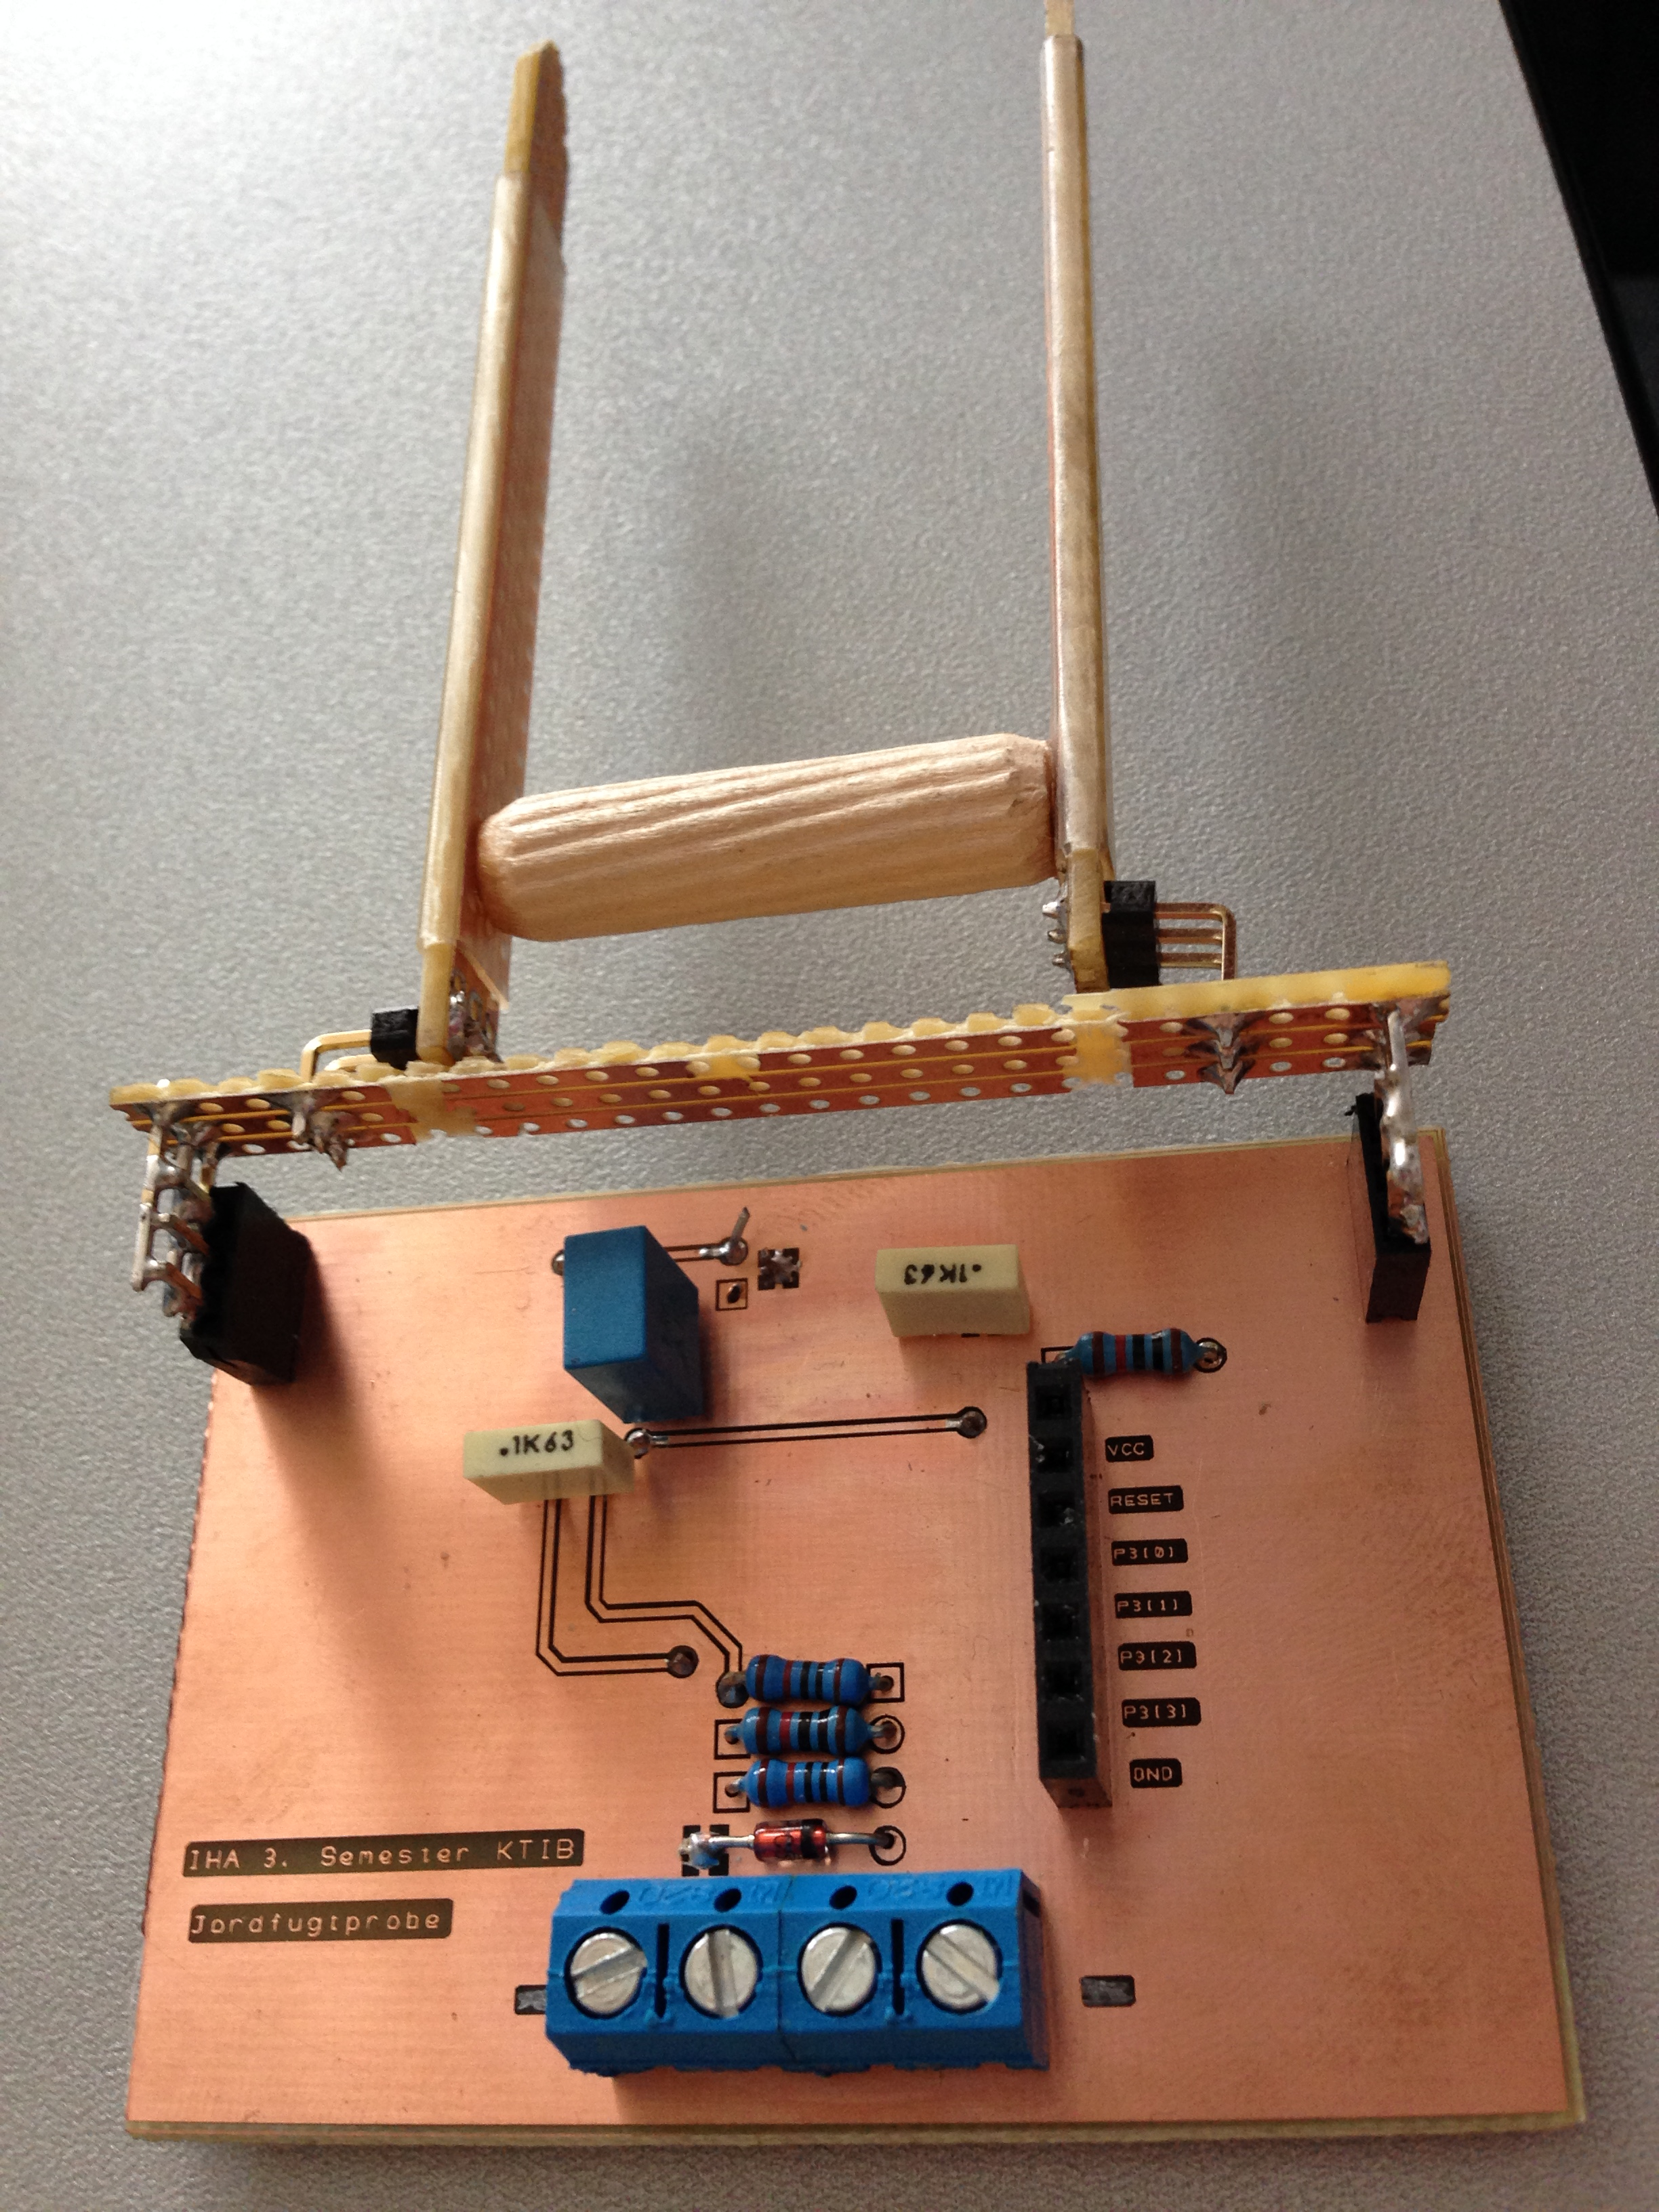
\includegraphics[scale=0.08]{HardwareArkitektur/Sensore/Jordfugt_billeder/print_ny_top.JPG}
	\caption{Det nye print set fra oven}
	\label{photo:print_ny_top}
\end{figure} 

\begin{figure}[H]
	\centering 
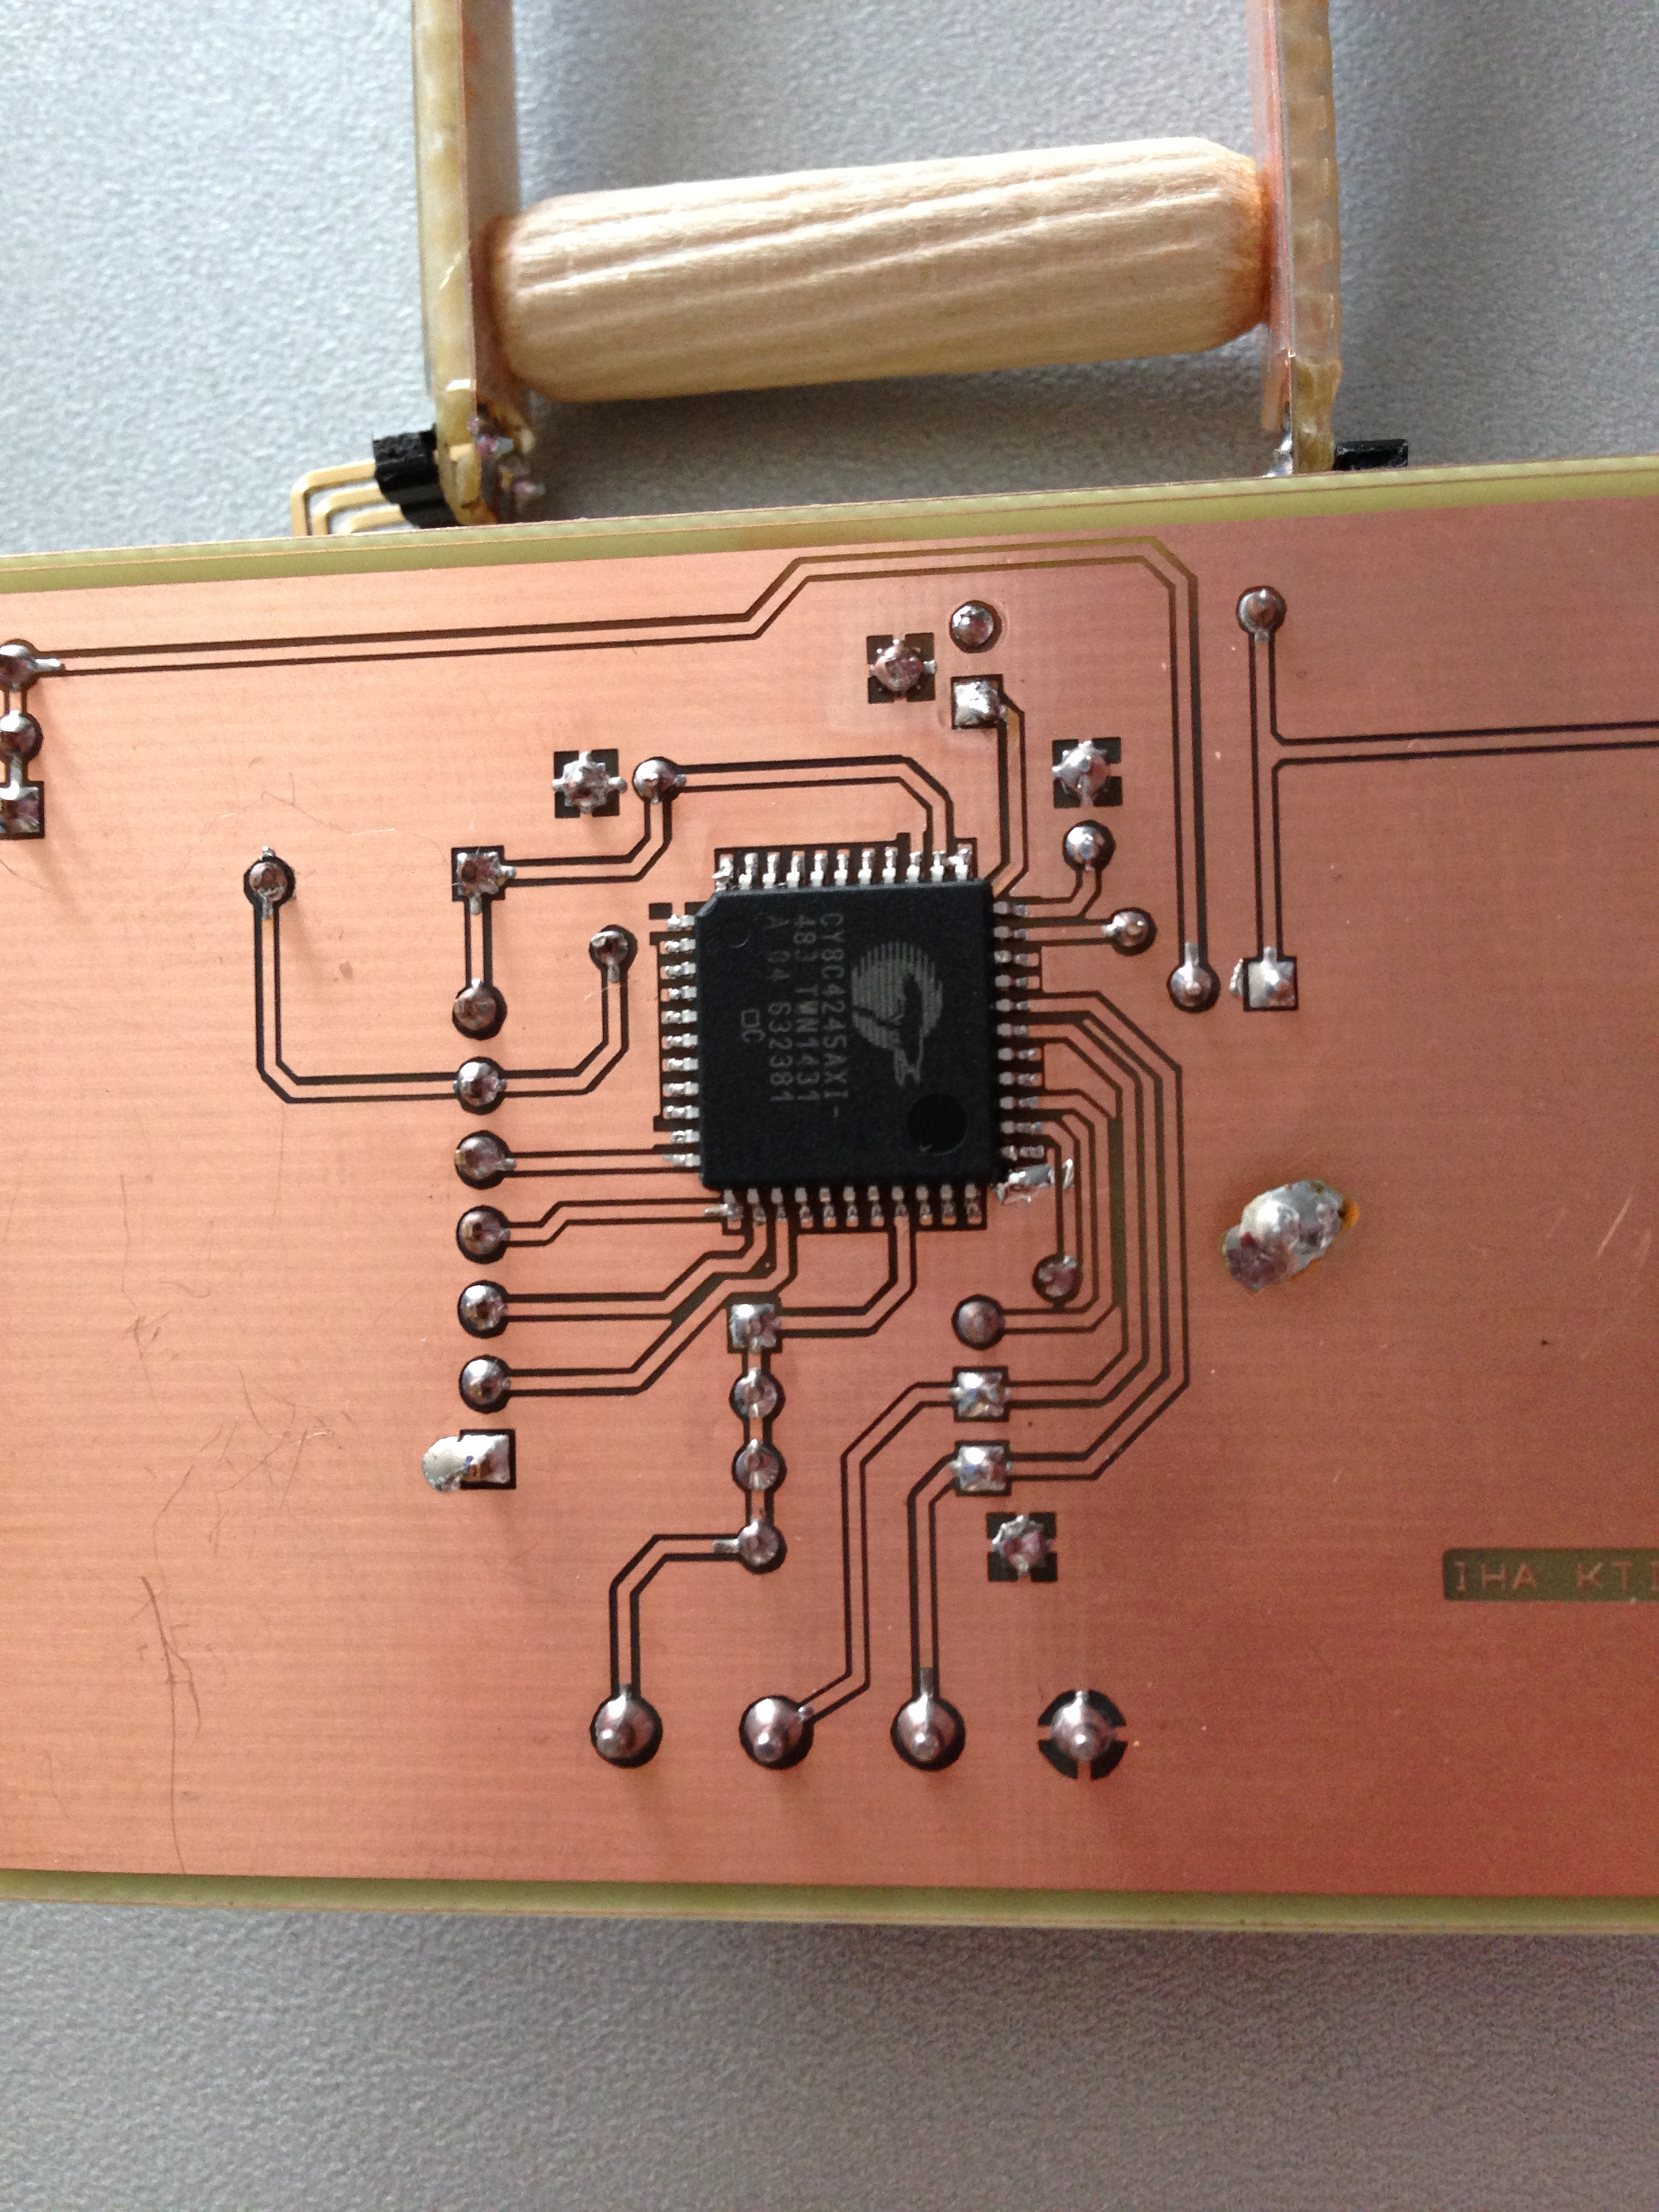
\includegraphics[scale=0.08]{HardwareArkitektur/Sensore/Jordfugt_billeder/print_ny_bund.JPG}
	\caption{Det nye print set fra bunden}
	\label{photo:print_ny_bund}
\end{figure} 

\begin{figure}[H]
	\centering 
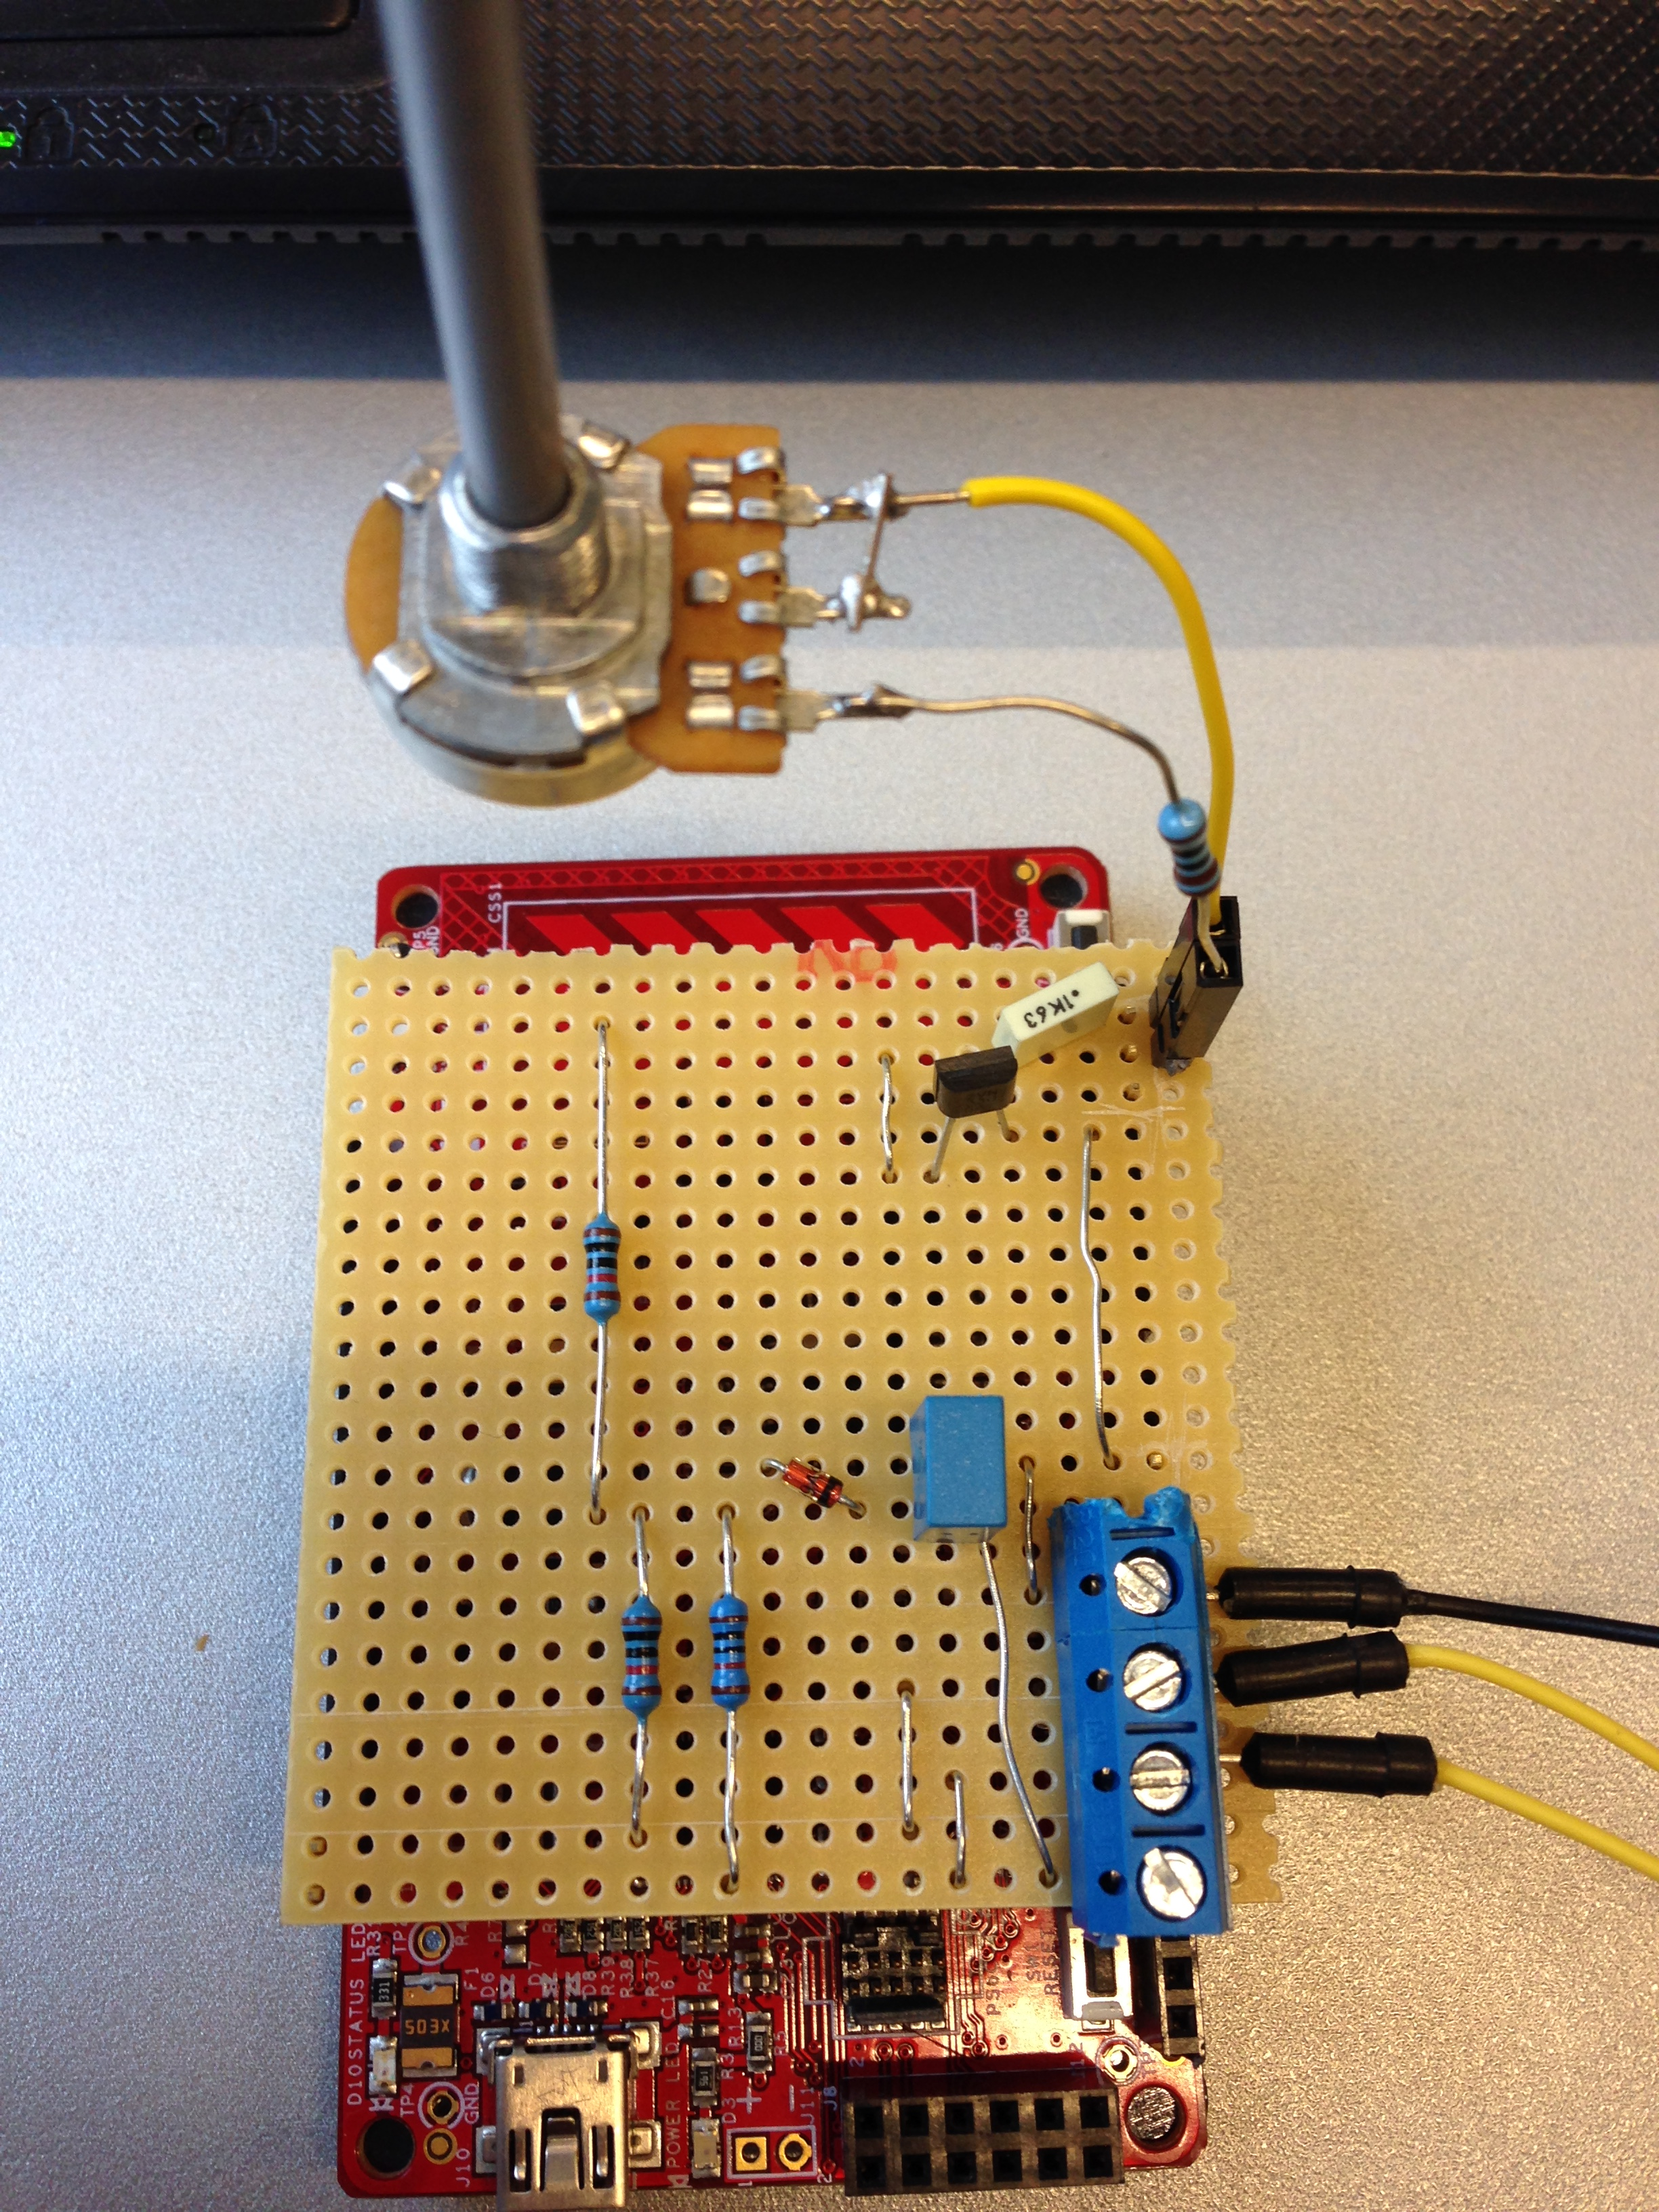
\includegraphics[scale=0.08]{HardwareArkitektur/Sensore/Jordfugt_billeder/shield.JPG}
	\caption{Shield. Potientiometeret emulerer proben}
	\label{photo:shield}
\end{figure} 

Vi kørte en test med det nye shield og da dette virkede var designet af jordfugtsensoren færdig. 
